\documentclass{article}

% ── NeurIPS 2026 Evaluations & Datasets Track ─────────────────────────────────
% Double-blind submission (default for evaluation papers)
\usepackage[eandd]{neurips_2026}
% Camera-ready: \usepackage[eandd, final]{neurips_2026}

% ── Packages ──────────────────────────────────────────────────────────────────
% Note: geometry and times are loaded by neurips_2026.sty; do not re-load them.
\usepackage{booktabs}
\usepackage{microtype}
\usepackage{graphicx}
\usepackage{hyperref}
%% math_commands.tex — shared notation for Shift-Specific STGNN Robustness

\usepackage{amsmath,amssymb,amsfonts}
\usepackage{bm}

% General math
\newcommand{\R}{\mathbb{R}}
\newcommand{\E}{\mathbb{E}}
\DeclareMathOperator*{\argmin}{arg\,min}
\DeclareMathOperator*{\argmax}{arg\,max}

% Graph notation
\newcommand{\calG}{\mathcal{G}}          % graph
\newcommand{\calV}{\mathcal{V}}          % vertex set
\newcommand{\calE}{\mathcal{E}}          % edge set
\newcommand{\Aadj}{\mathbf{A}}           % adjacency matrix
\newcommand{\Aadapt}{\hat{\mathbf{A}}}  % adaptive adjacency
\newcommand{\Dfixed}{\tilde{\mathbf{D}}} % degree matrix

% Signal / time-series
\newcommand{\xvec}{\mathbf{x}}           % input signal
\newcommand{\yvec}{\mathbf{y}}           % target
\newcommand{\hvec}{\mathbf{h}}           % hidden state
\newcommand{\Eset}{\mathcal{S}}          % sensor set
\newcommand{\Emask}{\mathcal{M}}         % dropout mask

% Shift notation
\newcommand{\DeltaCity}{\Delta_{\text{city}}}
\newcommand{\DeltaSensor}{\Delta_{\text{sensor}}}
\newcommand{\DeltaTemp}{\Delta_{\text{temp}}}
\newcommand{\DSRC}{\mathcal{D}_{\text{src}}}   % source domain
\newcommand{\DTGT}{\mathcal{D}_{\text{tgt}}}   % target domain

\usepackage{cleveref}

% ── Document ──────────────────────────────────────────────────────────────────
\title{How Adaptive Traffic Models Redistribute Fragility:\\
       A Multi-Shift Diagnostic of Spatiotemporal Architectures}

\author{Anonymous Authors}

\begin{document}
\maketitle

\begin{abstract}
Spatiotemporal graph neural networks (STGNNs) dominate traffic forecasting benchmarks,
yet which architectural properties govern their robustness under realistic deployment
shifts remains unclear.
Eight frozen architectures are evaluated under three deployment-motivated shifts---inference-time
sensor dropout, zero-shot cross-city transfer (METR-LA\,$\to$\,PEMS-BAY), and
weekday/weekend temporal subgroup shift---with all predictions pre-registered before
any experiments ran.

Robustness turns out to be shift-specific, and architectural progress changes failure
modes rather than eliminating them.
Adjacency routing concentration, $\mathrm{max\_mass}(A)$, explains the sensor-dropout
ranking at Pearson $\rho{=}{+}0.979$ across all four adaptive models.
Graph WaveNet's dense softmax routing ($\mathrm{max\_mass}{\approx}0.23$) degrades
$4.3{\times}$ more than DCRNN under 30\% dropout; a mask-aware inference variant that
zeroes dropped-sensor adjacency entries recovers 75\% of the gap without retraining.
Sensor-dropout robustness is therefore not a property of topology learning per se, but of
routing density: AGCRN ($\mathrm{max\_mass}{=}0.008$) and STAEformer show fragility
comparable to DCRNN despite learning adaptive spatial relations.
Cross-city and temporal fragility lie on orthogonal axes: MegaCRN achieves the best
zero-shot city-transfer score yet exhibits $8$--$9{\times}$ larger temporal subgroup gaps
than the canonical bank---a fragility axis invisible in five-model evaluations and not
driven by explicit temporal covariates in MegaCRN (mechanism ablations,
\S\ref{sec:mechanism}).
Deployment-oriented model selection should be based on the target shift type and routing
density of candidate architectures, not on in-distribution accuracy alone.

\end{abstract}

\section{Introduction}
\label{sec:intro}

Traffic forecasting underpins urban services---ride-hailing dispatch, signal
timing, congestion management---and STGNNs are the dominant
tool~\citep{li2018dcrnn,wu2019gwnet,yu2018stgcn}. In the lab, these models are
evaluated on held-out data from the same city, sensors, and time window as
training. Deployment conditions differ: sensors fail, models trained in one
city are applied to another, and traffic shifts between weekdays and weekends.
Which architectures hold up under these shifts is a deployment question that
in-distribution accuracy cannot answer.

Prior STGNN robustness work emphasizes synthetic
corruptions~\citep{zhang2025strap} or frames cross-city transfer as few-shot
learning~\citep{zeng2025fedtt,jing2026tlgpstgn}. Missing is a controlled
\emph{diagnostic} study that (i) uses deployment-realistic shifts, (ii)
evaluates the same frozen backbone under multiple shifts, (iii) attributes
differences to specific architectural choices, and (iv) pre-registers
hypotheses so refuted predictions carry the same evidential weight as
confirmed ones. Cross-city comparisons also conflate transfer difficulty with
inductive bias---adaptive models can re-learn target topology, fixed models
cannot---which a matched-structural-access protocol (source-city topology for
all backbones) removes. No prior study systematically compares how different
adaptive-relation designs---GWNet's dense softmax routing, MegaCRN's
meta-graph memory, STAEformer's adaptive embeddings---redistribute fragility
across deployment shifts.

We assemble a bank of eight architectures trained on METR-LA---a five-model
canonical bank spanning graph-free (GRU), fixed-graph (DCRNN, STGCN), and
adaptive-graph (MTGNNLight, GWNet), plus three modern adaptive-relation models
(AGCRN, MegaCRN, STAEformer)---and evaluate each frozen checkpoint under three
shifts: \textbf{sensor dropout} (10--50\% zeroed at inference, 5 random masks),
\textbf{cross-city transfer} (zero-shot METR-LA $\to$ PEMS-BAY under
matched structural access), and \textbf{temporal shift} (weekend vs.\ weekday
windows within the METR-LA test set).

Three findings stand out:
\begin{enumerate}
  \item No architecture dominates all three shifts; rankings change
        qualitatively between shift types. GWNet's dense adaptive adjacency
        is most fragile under sensor dropout (${\sim}4.3{\times}$ worse than
        DCRNN at 30\%) but not the worst at city transfer. DCRNN leads
        cross-city in the canonical bank; MegaCRN overtakes it once the
        extended set is added.

  \item GWNet's dropout fragility is the visible tail of a routing-density
        relation: $\mathrm{max\_mass}(A)$ ranks $\Delta_{\mathrm{sensor}}$ at
        Pearson $\rho{=}{+}0.979$ over four adaptive backbones on METR-LA,
        replicating at $\rho{=}{+}0.910$ on PEMS04 with native checkpoints.
        Replacing the learned adjacency with a fixed road graph cuts dropout
        sensitivity by 46\%; a mask-aware variant recovers 75\% without
        retraining. AGCRN ($\mathrm{max\_mass}{=}0.008$) and STAEformer match
        DCRNN despite learning adaptive relations: the operative factor is
        routing density, not topology learning.

  \item Modern adaptive-relation models distribute their failures across axes.
        AGCRN and STAEformer survive sensor dropout; MegaCRN leads cross-city.
        But MegaCRN and STAEformer carry weekday/weekend gaps
        ${\sim}8$--$9{\times}$ the canonical bank---an axis that the
        five-model evaluation could not have surfaced, and one that explicit
        TOD/DOW covariates do not explain
        (Section~\ref{sec:mechanism}).
\end{enumerate}

Sixteen predictions were pre-registered in five stages, each frozen before
the next round of training (ledger and confirmed/refuted/partial criteria:
Appendix~\ref{sec:appendix_preregistered}). Four were refuted: GWNet's
dominant failure axis was predicted to be cross-city transfer, not sensor
dropout; temporal fragility was predicted to be architecture-invariant, but
is not---findings invisible in a confirmation-only evaluation. Three
follow-ups---PEMS04-native routing-density replication
(Appendix~\ref{sec:appendix_pems04_routing}), the mask-aware dropout-ratio
sweep (Appendix~\ref{sec:appendix_mask_aware_sweep}), and cross-city
zero-padding sensitivity (Appendix~\ref{sec:appendix_no_pad_sensitivity})---are
flagged as reviewer-driven, reported alongside the pre-registered core. The
frozen-checkpoint protocol is reproducible end-to-end on a single commodity
GPU; checkpoints are released as supplementary material.

\section{Related Work}
\label{sec:related}

\paragraph{Spatiotemporal graph neural networks for traffic.}
DCRNN~\citep{li2018dcrnn} introduced bidirectional diffusion convolution
inside a recurrent encoder-decoder. Graph WaveNet~\citep{wu2019gwnet}
replaced the fixed graph with a learned adaptive adjacency.
STGCN~\citep{yu2018stgcn} alternates gated temporal convolutions with spectral
graph convolutions. A plain GRU is the graph-free baseline; MTGNNLight adds a
sparse adaptive topology. These five form our canonical bank. Inductive
alternatives like MTGNN~\citep{wu2020mtgnn} and AGCRN~\citep{bai2020agcrn}
infer graph structure from data, while newer adaptive-relation
models---MegaCRN~\citep{jiang2023megacrn} (meta-graph memory with temporal
covariates) and STAEformer~\citep{liu2023staeformer} (Transformer with
spatial-temporal adaptive embedding)---now top traffic leaderboards. We
include the MTGNN-inspired light variant in the canonical evaluation, and
extend the diagnostic to AGCRN, MegaCRN, and STAEformer for external
validity. Our results show that MTGNNLight's sparser learned graph reduces
but does not eliminate sensor-dropout fragility relative to GWNet's dense
softmax product graph, while AGCRN and STAEformer match DCRNN under sensor
dropout---which points to adjacency density and routing design (not
topology-learning per se) as the source of GWNet's routing brittleness.
None of these architectures were previously evaluated for robustness under
deployment-time distribution shift; the published numbers are
in-distribution held-out accuracy only.

\paragraph{Distribution shift in spatiotemporal models.}
A handful of recent methods address distribution shift in STGNNs.
STRAP~\citep{zhang2025strap} handles spatio-temporal OOD scenarios with
retrieval-augmented pattern learning: at inference, it retrieves historical
patterns from a stored library and injects them via a plug-and-play prompt,
adapting the model without re-training. TL-GPSTGN~\citep{jing2026tlgpstgn}
prunes graph context with information-theoretic criteria during training to
improve OOD generalization. These propose interventions; our work provides a
diagnostic---which backbones degrade under which shifts and why---a
prerequisite for designing targeted retrieval, topology-aware, or
imputation-based responses.

\paragraph{Cross-city transfer learning.}
Several papers frame cross-city generalization as few-shot or federated
learning. FedTT~\citep{zeng2025fedtt} trains a federated model across
multiple cities with traffic-view imputation and a domain adapter for
cross-city discrepancies. CAST-CKT~\citep{fofanah2026castckt} uses
chaos-aware attention and adaptive topology learning for cross-city
knowledge transfer. The LargeST benchmark~\citep{liu2023largest} ships with
a traffic-pattern bank retrieved by pattern matching. All of these use some
target-city data at training or adaptation time. We instead evaluate the
zero-shot case: models trained only on METR-LA applied directly to PEMS-BAY,
no adaptation---the setting that arises whenever a target city has no
historical data.

\paragraph{Topology-agnostic and foundation-model approaches.}
UniSTOK~\citep{anonymous2025unistok} tokenizes spatiotemporal signals
uniformly across variable sensor configurations; topology-free foundation
models like Chronos-2~\citep{ansari2024chronos} discard the graph entirely.
Cross-city foundation models train on many cities and adapt by fine-tuning,
which again needs target-domain data. Our zero-shot setting is
complementary: it asks which architectural properties confer robustness
before any adaptation is available---a prerequisite for deciding when
topology-agnostic or fine-tuning approaches are worth the trouble.

\paragraph{Sensor failure and data imputation.}
Mask-aware reconstruction architectures like GRIN~\citep{cini2022grin} and
BRITS~\citep{cao2018brits} explicitly reconstruct missing inputs before or
during graph aggregation. We ask the orthogonal question: among standard
STGNNs without imputation, which architectural choices confer robustness and
which amplify fragility? The answer reveals architecture-intrinsic failure
modes that imputation-based and foundation-model approaches would otherwise
mask. Our LOCF baseline (Appendix) confirms that temporal carry-forward
largely eliminates the fragility ranking, so the sensor-dropout findings are
specific to the silent zero-masking scenario.

\section{Problem Setup and Backbone Bank}
\label{sec:setup}

The audit evaluates eight frozen STGNN checkpoints under three
deployment-realistic shifts. Table~\ref{tab:audit_design} summarizes each
shift axis, its metric, the protocol control, the main validity threat, and
the appendix that addresses it.

\begin{table}[H]
\centering
\caption{\textbf{Audit design at a glance.} Three deployment-realistic shifts evaluated
under a unified frozen-checkpoint protocol.}
\label{tab:audit_design}
\vskip 0.05in
\small
\begin{tabular}{p{2.3cm}p{2.6cm}p{2.6cm}p{2.8cm}p{1.5cm}}
\toprule
\textbf{Shift axis} & \textbf{Metric} & \textbf{Control} & \textbf{Validity threat} & \textbf{App.\ check} \\
\midrule
Sensor dropout &
  $\DeltaSensor$: MAE delta (norm.) &
  MAE on kept sensors only; primary mask &
  Random vs.\ structured dropout pattern &
  \ref{sec:appendix_structured_dropout}, \ref{sec:appendix_multimask} \\
Cross-city transfer &
  X-city norm.\ MAE &
  Matched structural access (source adj) &
  Subset sampling; padding inflation &
  \ref{sec:appendix_subset_sensitivity}, \ref{sec:appendix_no_pad_sensitivity} \\
Temporal subgroup &
  $\DeltaTemp$: weekend$-$weekday (norm.; mph comparison) &
  Within-split stratification; no new data &
  Metric-dependent sign reversal &
  \ref{sec:appendix_temporal_absolute}, \ref{sec:appendix_temporal_cov} \\
\bottomrule
\end{tabular}
\end{table}

\paragraph{How to read the audit.}
Each column in the main tables is an estimand, not a single leaderboard score.
Clean MAE identifies the checkpoint being audited. $\DeltaSensor$ measures
incremental damage from silent zero-masking on the source city. Cross-city MAE
measures zero-shot transfer under matched structural access, and $\DeltaTemp$
measures a weekday/weekend subgroup gap inside the held-out source-city test
split. We therefore compare models within a shift axis and treat changes in
rank across axes as the object of study. This convention also avoids turning
the masked-MAE convention used by newer adaptive-relation models into a false
clean-performance comparison with the canonical bank.

\subsection{Backbone Architectures}
\label{subsec:backbones}

The canonical bank covers five architectures from graph-free to fixed-graph to
adaptive-graph.

\textbf{DCRNN}~\citep{li2018dcrnn} uses a bidirectional diffusion GRU on a
fixed road-distance adjacency $\Aadj$ (truncated at $K$ hops in both
directions), fixed at training and inference.
\textbf{Graph WaveNet (GWNet)}~\citep{wu2019gwnet} adds a learned adaptive
adjacency
\begin{equation}
  \Aadapt = \text{softmax}(\mathbf{E}_1 \mathbf{E}_2^\top),
  \label{eq:adaptive_adj}
\end{equation}
with $\mathbf{E}_1, \mathbf{E}_2 \in \mathbb{R}^{N \times d_e}$ trained end-to-end and tied to the $N$ training nodes.
\textbf{STGCN}~\citep{yu2018stgcn} alternates gated temporal convolutions with
truncated-Chebyshev spectral graph convolutions over the same fixed road
adjacency.
\textbf{GRU} is a graph-free recurrent baseline that treats the $N$ sensors as
a single feature vector and uses no adjacency.
\textbf{MTGNNLight} is a lightweight MTGNN variant~\citep{wu2020mtgnn} that
learns a sparse adaptive graph via pairwise cosine similarity on a single
embedding $\mathbf{E}\in\mathbb{R}^{N\times d}$ and keeps only top-$k$
neighbors per node. This directly contrasts with GWNet's dense all-pairs
softmax and isolates whether dropout fragility depends on adjacency density or
on topology learning per se (P14).

These five share a unified config (hidden dim 64, seq/pred 12, Adam $1{\times}10^{-3}$,
weight decay $10^{-4}$, cosine schedule, 100 epochs, patience 15). To rule out
training-artifact explanations of GWNet's fragility, we additionally train
\textbf{GWNet[CM]} (patience 30) and \textbf{GWNet[Strong]} (P17; hidden 128,
adaptive embed 20, patience 30); both are frozen at shift-eval time.

\subsection{Backbone Bank Protocol}
\label{subsec:bank}

We train each backbone once on METR-LA~\citep{li2018dcrnn} using the
chronological 70/10/20 split and three fixed seeds. The resulting checkpoints
are frozen before any shift evaluation: no model is re-trained, fine-tuned, or
selected separately for sensor dropout, cross-city transfer, or temporal
subgroup analysis.
An additional four-backbone few-shot probe relaxes this constraint to test
limited target-data adaptation (Appendix~\ref{sec:appendix_fewshot}).

Table~\ref{tab:main} reports the clean METR-LA MAE together with the three
shift metrics. The clean column is included only to anchor the starting point
of each checkpoint. Our claims are not based on clean ranking: a backbone can
be useful for diagnosing a failure mechanism even when it is not the strongest
source-city forecaster. For the same reason, GWNet[CM] and GWNet[Strong] are
treated as control checkpoints for the GWNet finding, not as additional entries
in the main bank.

\subsection{Extended adaptive-relation models}
\label{subsec:extended_models}

To probe generality, we add three architectures using the same METR-LA split
and frozen-checkpoint rule:
\textbf{AGCRN}~\citep{bai2020agcrn} (node-adaptive GRU, no temporal
covariates); \textbf{MegaCRN}~\citep{jiang2023megacrn} (meta-graph memory
with TOD/DOW inputs); \textbf{STAEformer}~\citep{liu2023staeformer}
(Transformer with spatial-temporal adaptive embeddings encoding temporal
covariates). These models use their standard masked-MAE convention, while the
canonical bank uses plain MAE; Table~\ref{tab:extended} reports clean values
only to identify checkpoints, not to rank clean performance across families.

\subsection{Distribution shifts}
\label{subsec:shifts}

\paragraph{Sensor dropout.}
At inference, a random 30\% of sensor channels are zero-masked. We do not
re-instantiate the 207-node model; it sees a 207-dimensional input with zeroed
channels, and MAE is computed on the kept sensors only so clean and masked
evaluations are directly comparable. Tables~\ref{tab:main}--\ref{tab:extended}
report the pre-registered primary-mask aggregate; Appendix~\ref{sec:appendix_multimask}
reports 5-mask aggregates to separate mask-sampling from model-weight variance.
GRU is the main mask-sampling caveat. Structured dropout patterns
(hub and contiguous) are in Appendix~\ref{sec:appendix_structured_dropout}.
This protocol isolates silent failure; the LOCF comparison in
Appendix~\ref{sec:appendix_imputation} shows that effective imputation can
largely remove the zero-mask gap.
Supplementary probes add stale hold, noise, bias, and intermittent missingness
(Appendix~\ref{sec:appendix_corruption_suite}).

\paragraph{Cross-city transfer.}
The frozen METR-LA model is evaluated zero-shot on
PEMS-BAY~\citep{li2018dcrnn} (Bay Area, 325 sensors, 52,116 timesteps).
A second pair (PEMS04 source, 307 sensors; zero-shot on METR-LA and PEMS-BAY)
is in Appendix~\ref{sec:appendix_pems04} for cross-city generality (P18).
``Zero-shot'' means no re-training or fine-tuning. Because PEMS-BAY has 325
sensors and the METR-LA checkpoints have 207 input channels, we subsample 207
PEMS-BAY sensors (5 subsets); rankings remain stable at 150-node coverage
(Appendix~\ref{sec:appendix_subset_sensitivity}).

\textbf{Matched structural access (canonical comparison).}
The main cross-city comparison uses source-only adjacency: every backbone
uses the METR-LA adjacency at inference, removing the asymmetry that
adaptive-graph models cannot access target topology by construction.
Under this constraint, any observed advantage is architectural, not an
artifact of privileged topology access
(target-adj results: Appendix~\ref{sec:appendix_source_adj}).
MAE is normalized with source-city statistics for cross-architecture
comparability.

\paragraph{Temporal subgroup shift.}
METR-LA spans weekdays and weekends with different traffic patterns; the
model is trained on both. We stratify the test set by day type---weekday
(5,104 windows) and weekend (1,728 windows)---and report
$\DeltaTemp = \mathrm{MAE}_{\text{weekend}} - \mathrm{MAE}_{\text{weekday}}$.
This is a subgroup performance gap within the existing test split, not
deployment to a new time window. In addition to the normalized gaps, we report
the extended models' masked-mph gaps on the same checkpoints and windows
(Appendix~\ref{sec:appendix_temporal_absolute}). The latter exclude zero-valued
targets, whereas normalized MAE includes all targets; the comparison changes
both scaling and the target mask.

\paragraph{Protocol summary.}
{\small Train on METR-LA (207 sensors, 5-min, 70/10/20 split); 3 seeds,
100 epochs, patience 15; frozen at evaluation. \emph{Sensor:} 30\% silent
primary zero-mask for Tables~\ref{tab:main}--\ref{tab:extended}, MAE on kept sensors.
\emph{City:} zero-shot to
PEMS-BAY (325$\to$207 subsampled, 5 subsets), source-only adjacency
(matched-structural-access; padding sensitivity in
Appendix~\ref{sec:appendix_no_pad_sensitivity}). \emph{Temporal:} weekday
(5{,}104) vs.\ weekend (1{,}728) test windows. \emph{Aggregation:}
mean$\,\pm\,$population std over 3 seeds unless a table explicitly reports
multi-mask summaries;
METR-LA train-statistics normalization for the canonical bank,
model-specific scaler for extended models
(\S\ref{subsec:extended_models}).}

\section{Results across Test Conditions}
\label{sec:taxonomy}

\paragraph{Pre-registered hypotheses.}
We pre-registered 16 predictions in five stages before running the corresponding experiments.
Of these, 10 were confirmed, 4 were refuted, and 2 were partially confirmed.
Appendix~\ref{sec:appendix_preregistered} lists the predictions and outcomes; the corresponding experiment identifiers (P14--P19, P21) accompany the results below.

Table~\ref{tab:main} reports the main results across all five backbones and three shift types.
Each column measures a different response to the test conditions. We examine how model ordering changes between columns.

\begin{table}[H]
\centering
\caption{\textbf{Robustness rankings are shift-specific.}
Five backbones evaluated across sensor dropout, cross-city transfer, and
temporal subgroup shift. Values are mean $\pm$ population std over 3 seeds;
lower is better.}
\label{tab:main}
\vskip 0.05in
\resizebox{\linewidth}{!}{%
\begin{tabular}{lcccc}
\toprule
\textbf{Backbone} & \textbf{In-dist MAE (mph)} & \textbf{$\DeltaSensor$ (30\%, norm.)} & \textbf{X-city (norm.)$^{\dagger}$} & \textbf{$\DeltaTemp$ (norm.)} \\
\midrule
DCRNN (fixed diffusion)       & $6.58 \pm 0.03$ & $+0.020 \pm 0.002$ & $0.180 \pm 0.001$ & $+0.087 \pm 0.004$ \\
GRU   (graph-free)            & $7.49 \pm 0.12$ & $+0.025 \pm 0.012$ & $0.278 \pm 0.009$ & $+0.093 \pm 0.003$ \\
MTGNNLight (sparse cosine-sim)& $6.88 \pm 0.11$ & $+0.051 \pm 0.012$ & $0.244 \pm 0.004$ & $+0.075 \pm 0.007$ \\
STGCN (fixed spectral)        & $7.12 \pm 0.05$ & $+0.078 \pm 0.007$ & $0.249 \pm 0.008$ & $+0.093 \pm 0.003$ \\
GWNet (dense adaptive adj)    & $7.85 \pm 0.11$ & $+0.088 \pm 0.017$ & $0.268 \pm 0.006$ & $+0.094 \pm 0.009$ \\
\bottomrule
\end{tabular}}
{\footnotesize $^{\dagger}$Source-only adjacency; METR-LA-stat normalized MAE on PEMS-BAY.}
\end{table}

\paragraph{Sensor dropout.}
GWNet has the largest sensor-dropout increase in the canonical bank. DCRNN and
GRU have the smallest deltas, while MTGNNLight is markedly less fragile than
GWNet despite also learning topology. Learning a graph is therefore not enough to explain the fragility;
the relevant contrast is sparse learned routing versus dense all-pairs softmax. Capacity controls reduce but do not remove the GWNet
gap (Table~\ref{tab:consolidated}; Appendix~\ref{sec:appendix_stronger_gwnet}).
Dropping high-degree sensors increases GWNet's gap but reduces DCRNN's. This difference is consistent with GWNet relying more heavily on routes through these sensors.
The ranking also depends on corruption type: at 30\% affected channels,
GWNet's healthy-sensor increase is $+0.16$ mph for noise but $+1.96$ mph
for bias, compared with DCRNN's $+0.28$ and $+1.00$ mph, respectively
(Appendix~\ref{sec:appendix_corruption_suite}).

\paragraph{Cross-city transfer under matched structural access.}
Under source-only adjacency, DCRNN is the strongest canonical-bank transfer
baseline. STGCN, also a fixed-graph model, loses much of its advantage when target topology is withheld and then performs similarly to GWNet. The DCRNN advantage also holds on a second
city pair, while padding sensitivity changes absolute MAE but not the ordering
(Table~\ref{tab:consolidated}; Appendix~\ref{sec:appendix_no_pad_sensitivity}).
The GRU baseline is useful here because it removes graph mismatch entirely and
still transfers worst in the canonical bank. Cross-city robustness therefore
does not come from ignoring structure; it depends on how the source-city
structure is used when the target graph is unavailable. A limited fine-tuning comparison is reported in Appendix~\ref{sec:appendix_fewshot}.

\paragraph{Temporal subgroup shift (canonical bank).}
The canonical models have similar weekend/weekday gaps, with much less separation than under sensor dropout or city transfer. None uses explicit time-of-day or day-of-week inputs, and graph type does not explain the small differences. The extended models show larger differences whose interpretation depends on the error metric (\S\ref{sec:extended}).

Appendix Table~\ref{tab:consolidated} summarizes the capacity, source-adjacency, structured-dropout, and horizon comparisons.

\subsection{AGCRN, MegaCRN, and STAEformer}
\label{sec:extended}

Table~\ref{tab:extended} compares AGCRN, MegaCRN, and STAEformer with DCRNN. All use the same METR-LA split and remain frozen during evaluation.

\begin{table}[H]
\centering
\caption{\textbf{Adaptive-relation models under the three test conditions.}
Clean MAE follows each architecture's standard masked-MAE convention; shift
columns use the same normalized protocol as Table~\ref{tab:main}.}
\label{tab:extended}
\vskip 0.05in
\resizebox{\linewidth}{!}{%
\begin{tabular}{lcccc}
\toprule
\textbf{Model} & \textbf{Clean MAE (mph)} & \textbf{$\DeltaSensor$ (30\%, norm.)} & \textbf{Cross-city (src, norm.)} & \textbf{$\DeltaTemp$ (norm.)} \\
\midrule
AGCRN      & $4.09 \pm 0.02^{\dagger}$ & $+0.019 \pm 0.001$ & $0.206 \pm 0.009$ & $+0.061 \pm 0.008$ \\
MegaCRN    & $3.04 \pm 0.06^{\dagger}$ & $-0.048 \pm 0.027$ & $0.163 \pm 0.003$ & $+0.734 \pm 0.019$ \\
STAEformer & $2.93 \pm 0.01^{\dagger}$ & $+0.015 \pm 0.001$ & $0.223 \pm 0.008$ & $+0.750 \pm 0.003$ \\
\midrule
DCRNN (ref) & $6.58 \pm 0.03$ & $+0.020 \pm 0.002$ & $0.180 \pm 0.001$ & $+0.087 \pm 0.004$ \\
\bottomrule
\end{tabular}}
\vskip 0.05in
{\footnotesize $\dagger$ Masked MAE (target $> 0$); DCRNN uses plain MAE.
Cross-family clean-performance ranking is not meaningful due to this convention difference.}
\end{table}

\paragraph{Sensor dropout.}
AGCRN and STAEformer stay near DCRNN on sensor dropout, so GWNet's result
cannot be read as ``adaptive graphs are fragile.'' The distinction is dense
all-pairs softmax (Eq.~\ref{eq:adaptive_adj}) versus node-specific or
attention-mediated relations. MegaCRN's negative delta is non-monotonic in
dropout ratio and is attributed to adjacency-mediated smoothing toward a weekday prior (\S\ref{sec:polish_ablations}), not as direct dropout
robustness.

\paragraph{Cross-city transfer.}
MegaCRN attains the lowest source-stat cross-city MAE, so DCRNN's lead
in zero-shot transfer holds only within the canonical bank. AGCRN and STAEformer fall between DCRNN and GWNet.

\paragraph{Temporal subgroup shift.}
In physical units, MegaCRN and STAEformer have \emph{lower} weekend error:
their weekend-minus-weekday gaps are $-0.594\pm0.051$ and
$-0.612\pm0.002$ masked mph, respectively. AGCRN's gap is
$+0.750\pm0.013$ mph. The normalized gaps in Table~\ref{tab:extended} are
positive for all three models. Thus the large normalized gaps do not establish
greater physical-error fragility: scaling and target masking reverse the sign
for two models (Appendix~\ref{sec:appendix_temporal_absolute}). Covariate
interventions address the normalized gap, not this absolute-error ranking.

\paragraph{Comparison across shifts.}
The adaptive-relation models differ across deployment settings
(Figure~\ref{fig:shift_profiles}): AGCRN and STAEformer match DCRNN under
sensor dropout, MegaCRN leads source-normalized cross-city transfer, and
temporal comparisons depend on the reporting convention. Routing concentration
tracks sensor-dropout sensitivity even when clean accuracy and cross-city
ranking move in different directions. The sensor-dropout ranking is specific
to silent zero-masking; under last-observed-value carry-forward
(LOCF) with the true failure mask, the four backbones in the comparison recover
${\geq}97\%$ of the gap (Appendix~\ref{sec:appendix_imputation}), so the
practical impact of GWNet's fragility depends on the deployment pipeline's
imputation policy. The main conclusions are drawn from METR-LA as the source
city; PEMS04 is used only for targeted source-city replication, not as a full
third-source benchmark (\S\ref{sec:discussion}).

\begin{figure}[H]
\centering
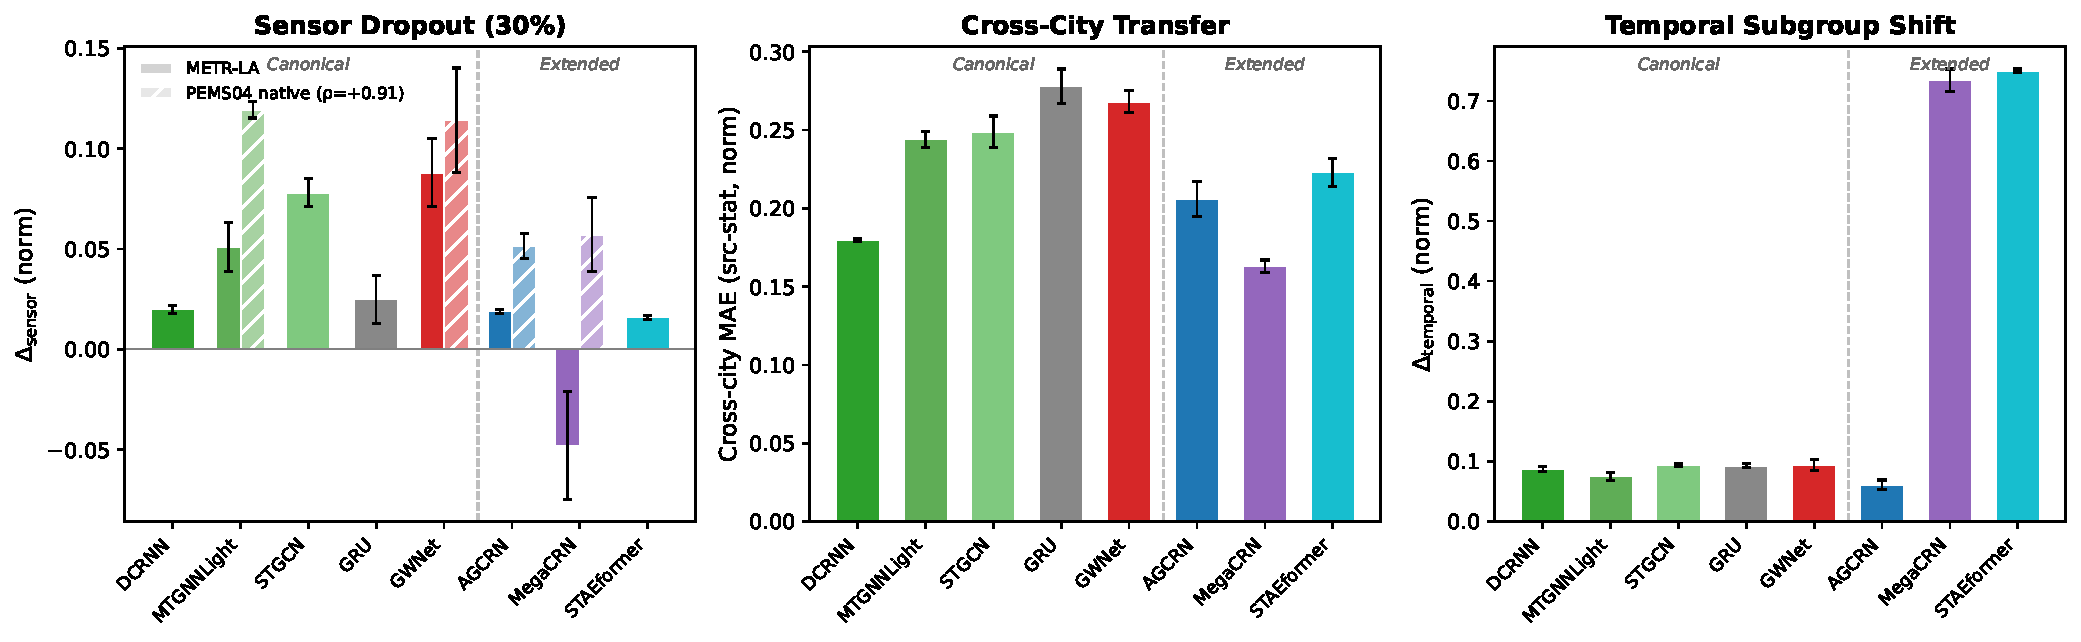
\includegraphics[width=\textwidth]{figures/shift_profiles.pdf}
\caption{\textbf{Sensor-dropout, transfer, and temporal errors.}
Sensor and city panels show all eight backbones; the dashed line separates
the canonical and extended banks. Hatched bars show PEMS04-native replication.
The temporal panel shows masked-mph gaps for the three extended models:
MegaCRN and STAEformer have lower weekend error despite positive normalized
gaps. Error bars are population std over three seed-level means.}
\label{fig:shift_profiles}
\end{figure}

\section{Mechanism: dense adaptive routing and sensor-dropout fragility}
\label{sec:mechanism}

The taxonomy shows GWNet's dense learned routing is fragile under sensor
dropout while AGCRN and STAEformer, which also learn adaptive spatial
relations, are not (Table~\ref{tab:extended}). Two questions follow: is the
dense adaptive adjacency (Eq.~\ref{eq:adaptive_adj}) the driver, and can the
failure mode be mitigated without retraining?

\subsection{Ablation: adaptive vs.\ fixed adjacency}

We run frozen GWNet checkpoints under two inference-time adjacency
configurations. \textbf{GWNet[adaptive]} keeps
$\Aadapt = \text{softmax}(\mathbf{E}_1 \mathbf{E}_2^\top)$;
\textbf{GWNet[fixed]} replaces $\Aadapt$ with the normalized METR-LA distance
adjacency $\Aadj$ and zeros out $\mathbf{E}_1, \mathbf{E}_2$ (rest of the
network unchanged).

\begin{table}[t]
\centering
\caption{\textbf{Replacing GWNet's adaptive adjacency with a fixed road graph halves
sensor-dropout sensitivity and improves city transfer by 22\%, at only 5\% in-distribution
cost.} Sensor dropout: 30\% zero-mask, 5 masks, 3 seeds. City MAE: target-adj, PEMS-BAY (mph),
reported here for interpretability; source-only normalized values in Appendix~\ref{sec:appendix_source_adj}.}
\label{tab:ablation}
\vskip 0.05in
\begin{tabular}{lccc}
\toprule
\textbf{Variant} & \textbf{In-dist MAE} & \textbf{$\DeltaSensor$ (30\%, multi-mask)} & \textbf{City MAE (mph)} \\
\midrule
GWNet[adaptive] & $7.85 \pm 0.11$ & $+0.092 \pm 0.030$ & $4.42 \pm 0.15$ \\
GWNet[fixed]    & $8.27 \pm 0.08$ & $+0.050 \pm 0.010$ & $3.44 \pm 0.04$ \\
\midrule
\emph{Change}   & $+5.3\%$        & $-45.7\%$          & $-22\%$         \\
\bottomrule
\end{tabular}
\end{table}

Fixed substitution cuts sensor-dropout sensitivity by $45.7\%$ and
city-transfer MAE by $22\%$, at $+5.3\%$ in-distribution cost---past the
pre-registered $\geq 30\%$ threshold for attributing fragility to the
adaptive adjacency. Per-horizon decomposition (Table~\ref{tab:consolidated})
shows GWNet's cross-city MAE is nearly horizon-flat ($+4\%$ growth
$h{=}1{\to}12$) while DCRNN grows $+46\%$: the transfer gap is static
structural mis-routing, not error accumulation.

\paragraph{Mask-aware adjacency variant.}
Zeroing and renormalizing adjacency rows/columns for dropped sensors at
inference ($\Aadapt[i,:]{=}\Aadapt[:,i]{=}0$, then
$\Aadapt \leftarrow \Aadapt / \max(\Aadapt\mathbf{1}, \epsilon)$) should
partially restore robustness without retraining.

\begin{table}[t]
\centering
\caption{\textbf{Mask-aware adjacency routing recovers 75\% of GWNet's sensor-dropout gap
without any retraining.} The intervention zeros and renormalizes adjacency rows/columns
for dropped sensors (${\sim}25$~LoC); both variants evaluated on kept sensors only (3 seeds,
5 random 30\% masks each).}
\label{tab:mask_aware}
\vskip 0.05in
\small
\begin{tabular}{lcc}
\toprule
\textbf{Variant} & \textbf{$\DeltaSensor$ (30\%, multi-mask)} & \textbf{Recovery} \\
\midrule
GWNet[standard]    & $+0.092 \pm 0.030$ & --- \\
GWNet[mask-aware]  & $+0.023 \pm 0.018$ & $75.2\%$ \\
\bottomrule
\end{tabular}
\end{table}

Mask-aware recovers $75.2\%$, beating fixed substitution at $45.7\%$:
selectively blocking only the affected rows/columns is better than replacing
the topology with a static prior. The intervention is ${\sim}25$ LoC and
deploys directly on existing GWNet checkpoints.

\subsection{Routing density as a shared mechanism hypothesis}
\label{sec:routing_spectrum}

The GWNet analysis above looks model-specific, but it is the visible tail of a
monotonic relation over \emph{all four} adaptive-graph models in our bank
($n{=}4$ adaptive backbones). Measuring adjacency concentration as
$\text{max\_mass}$ (mean per-row maximum probability) on METR-LA test samples
yields AGCRN $0.008$, MegaCRN $0.008$, MTGNN $0.16$, GWNet $0.23$. Pairing
with each model's $\DeltaSensor$ ($+0.011$, ${-}0.005$, ${+}0.051$,
${+}0.092$) gives Pearson $\rho{=}{+}0.979$ (over the four adaptive
backbones; Appendix~\ref{sec:appendix_routing_spectrum}).
Per-architecture adjacency proxies are canonical and averaged over rows,
samples, and three seeds; STAEformer has no single row-stochastic adjacency and
is excluded from the Pearson (full proxy definitions in
Appendix~\ref{sec:appendix_routing_spectrum}).
The relation replicates on PEMS04 with native checkpoints
($\rho{=}{+}0.910$ on the same four adaptive backbones, vs.\ $+0.979$ on
METR-LA; Appendix~\ref{sec:appendix_pems04_routing}); MegaCRN's
METR-LA-specific negative $\DeltaSensor$ becomes positive on PEMS04
($+0.057$), \emph{consistent with} (rather than fully confirming) the
weekday-prior smoothing diagnosis: a no-covariate retrain remains future
work (\S\ref{sec:discussion}). We treat the result as a two-city replicated
shared-mechanism \emph{hypothesis}, not a settled law.
Within GWNet, top-$k$ sparsification at inference traces the same curve:
relative fragility rises from $0.80\%$ at $k{=}10$ to $1.17\%$ at $k{=}\text{full}$
(Appendix~\ref{sec:appendix_density_sweep}). A first-order spectral bound on
zero-mask perturbation gives per-node corruption $\leq \lvert \mathcal{I} \rvert
\cdot \text{max\_mass}(A)$ up to constants, explaining the linear trend
(Appendix~\ref{sec:appendix_theory}).

\subsection{Ruling out two natural mechanism hypotheses}
\label{sec:polish_ablations}

Table~\ref{tab:mechanism_exclusion} reports ablations that progressively narrow
the cause of MegaCRN and STAEformer's temporal fragility; the final row is an
open residual, not a completed ablation.

\begin{table}[t]
\centering
\small
\caption{\textbf{Mechanism exclusion for MegaCRN/STAEformer temporal fragility.}
``Ruled out'' means the gap is unchanged or worsened after removing the hypothesized driver.}
\label{tab:mechanism_exclusion}
\vskip 0.05in
\begin{tabular}{p{2.6cm}p{3.2cm}p{3.0cm}p{2.5cm}}
\toprule
\textbf{Hypothesis} & \textbf{Test} & \textbf{Result} & \textbf{Verdict} \\
\midrule
TOD/DOW covariate channel
  & Randomize / swap embeddings at inference (5 seeds)
  & MegaCRN: $0\%$ gap change; STAEformer: $12.5\%$ reduction
  & Ruled out (MegaCRN); partial (STAEformer) \\[2pt]
Memory-bank regularization
  & \emph{memzero}: zero memory bank at inference
  & Gap deepens ($-0.075$ vs $-0.040$ at $r{=}0.3$)
  & Ruled out \\[2pt]
Adjacency-mediated smoothing (sensor axis)
  & \emph{attnonly}: identity adjacency
  & $\DeltaSensor$ eliminated across all~$r$
  & Confirmed driver \\[2pt]
Encoder dynamics (temporal axis)
  & ---
  & Open
  & Residual \\
\bottomrule
\end{tabular}
\end{table}

MegaCRN's apparent sensor robustness is adjacency-mediated smoothing toward a
weekday-dominated prior---failure masquerading as robustness
(Appendix~\ref{sec:appendix_memory_ablation}).
The residual temporal fragility lives in the memory bank or encoder dynamics
and is not isolated by inference-time interventions; isolating it requires a
no-covariate retraining, left to future work
(Appendix~\ref{sec:appendix_temporal_cov}).

\subsection{Severity, degree stratification, and imputation baselines}

GWNet is the most sensitive backbone at all five dropout ratios
(GWNet/DCRNN ratio grows $2.5\times \to 4.6\times$ from $10\%$ to $40\%$;
Appendix~\ref{sec:appendix_severity}). Its highest-degree quartile suffers
$\DeltaSensor{=}{+}0.121$ versus $+0.066$ for Q1 ($1.83\times$); DCRNN shows
no degree dependence (Appendix~\ref{sec:appendix_degree_stratification}).
Last-observed-value carry-forward (LOCF) recovers ${\geq}97\%$ of the zero-mask
gap across backbones---the ranking is specific to silent-failure zero-masking
(Appendix~\ref{sec:appendix_imputation}).

\section{Discussion}
\label{sec:discussion}

\paragraph{Deployment guidance.}
Within the shifts, source city, and masking model evaluated here, the results
suggest several practical choices.
Under silent-failure zero-mask dropout, DCRNN, AGCRN, and STAEformer degrade
much less than GWNet; the GWNet gap is tied to dense softmax routing and the
mask-aware variant recovers 75\% without retraining. For zero-shot cross-city
transfer on METR-LA/PEMS-BAY-style highway networks, MegaCRN and DCRNN
perform well. Weekday/weekend comparisons require an explicit metric: MegaCRN and
STAEformer have positive normalized gaps but negative masked-mph gaps.
Their normalized values alone should not drive temporal deployment guidance.

\paragraph{Implications for robustness evaluation.}
In our bank, the clean-test ranking changes under sensor dropout and only
partly predicts cross-city transfer. Richer relation learning is not uniformly
more robust; weaknesses appear on different axes. Benchmarks should therefore
report per-shift results alongside in-distribution accuracy. The GWNet controls
make simple optimizer failure an unlikely explanation for its fragility
(Table~\ref{tab:consolidated}).

\paragraph{Recommendation artifact.}
The released $2{\times}2{\times}2$ decision table maps sensor reliability,
city transfer, and weekend exposure to observed fragility and mitigations
(Appendix~\ref{sec:appendix_decision_tree}). It covers the eight-model bank
and demotes MegaCRN's smoothing-related negative sensor delta. Its temporal
axis uses normalized gaps. AGCRN, recommended for two weekend-exposed
profiles, has the only positive masked-mph weekend gap among the extended
models (Table~\ref{tab:temporal_absolute}); these cells should not be used to
choose models for physical-error performance.

\paragraph{Limitations.}
All datasets are highway loop-detector data. METR-LA is the main training
source, with PEMS-BAY and PEMS04 used for targeted replications; urban
arterials and probe data remain untested. The model set is not exhaustive
(e.g., ASTGCN~\citep{guo2019astgcn}, DSTAGNN~\citep{lan2022dstagnn}), and the
main results use three training seeds. Zero-shot transfer is a diagnostic
floor, not a deployment recommendation; the few-shot probe covers four
backbones and limited adaptation (Appendix~\ref{sec:appendix_fewshot}). The
weekday/weekend comparison is a subgroup analysis within one test split,
not an OOD test. Walk-forward evaluation remains future work, and the gap's
sign depends on normalization and target masking. The six-architecture
concentration correlation weakens on PEMS-BAY and PEMS04; interventions
support the link only for GWNet. MegaCRN's negative sensor delta reflects
adjacency-mediated smoothing, and TOD/DOW covariates alone do not explain
its normalized temporal gap.

\paragraph{Scope of the zero-mask diagnostic.}
Zero is a physically possible speed, so a zero reading alone cannot identify
failure. Corruptions are assigned by a failure mask, not by observed values;
valid zeros at kept sensors are not classified as failures. Both remedies
require identifying failed sensors: LOCF uses the true failure mask
(Appendix~\ref{sec:appendix_imputation}), and detector errors increase MAE for
mask-aware routing (Appendix~\ref{sec:appendix_mask_fpfn}). We did not test LOCF
under imperfect detection. The gap applies where failures go undetected,
telemetry is delayed, or carry-forward is unreliable.

\section{Conclusion}
\label{sec:conclusion}

The evaluated STGNNs respond differently to sensor failure, city transfer,
and weekday/weekend traffic. Routing concentration correlates with sensitivity
to silent zero-filling across six METR-LA-trained adaptive architectures
(Pearson $\rho{=}{+}0.974$), with weaker positive associations on PEMS-BAY
and PEMS04. In Graph WaveNet, modifying routes around known failed sensors
recovers $75\%$ of the dropout gap without retraining. MegaCRN achieves the
lowest source-normalized transfer error, while its weekday/weekend gap and
STAEformer's change sign between normalized error and masked mph. These
results show why model selection requires separate comparisons for the
expected failures, transfer conditions, and error metric.


\bibliographystyle{abbrvnat}
\bibliography{references}

\appendix

% ============================================================
\section{Pre-Registered Hypotheses}
\label{sec:appendix_preregistered}
% ============================================================

Table~\ref{tab:preregistered} records all 16 pre-registered predictions alongside
experimental outcomes. Predictions were added in five stages before running the
corresponding experiments.

\textbf{Hosting and criteria.}
The ledger is hosted in the project notebook
\texttt{RESEARCH\_JOURNEY\_DEFENSE.md} with stage-stamped entries; each stage
was committed before the next round of training or evaluation began. A
prediction is marked \emph{confirmed} ({\checkmark}) when its directional claim
\emph{and} any pre-stated quantitative threshold (e.g., ``$\geq 30\%$
reduction'') hold; \emph{refuted} ({\texttimes}) when either fails;
\emph{partial} when one holds and the other does not. Only secondary protocol
details---mask seed indices, reporting-horizon choice, and figure
formatting---were finalized post-hoc; the predictions themselves, including
quantitative thresholds and the model bank, were frozen at registration time.
The breakdown is ten confirmed, three refuted, and three partial; verbatim
re-statements are linked from each row of Table~\ref{tab:preregistered}.

\begin{table}[h]
\centering
\caption{Pre-registered hypotheses and outcomes. Confirmed ({\checkmark}) or refuted
(\texttimes) by experiment.}
\label{tab:preregistered}
\vskip 0.1in
\small
\begin{tabular}{p{6cm}p{5cm}c}
\toprule
\textbf{Prediction} & \textbf{Outcome} & \textbf{Result} \\
\midrule
GWNet fails hardest under city transfer (topology overfitting)
  & GWNet is worst under sensor dropout, not city transfer; GRU is worst at city transfer
  & \texttimes \\
Graph-based models are more robust than GRU to sensor dropout
  & GRU is nearly as robust as DCRNN at 30\%; adaptive graph hurts, fixed graph helps
  & Partial \texttimes \\
All models degrade on PEMS-BAY vs.\ METR-LA
  & Source-stat MAE improves on PEMS-BAY (simpler traffic); target-stat reveals real gaps
  & \texttimes \\
Adaptive adjacency drives sensor-dropout fragility ($\geq$30\% reduction when ablated)
  & 43.1\% reduction confirmed
  & {\checkmark} \\
Temporal shift magnitude differs across architectures
  & All architectures within one std of each other
  & \texttimes \\
STGCN (fixed spectral adj) $\DeltaSensor \leq$ DCRNN (fixed diffusion adj)
  & STGCN $+0.078$ $>$ DCRNN $+0.020$; but both $<$ GWNet $+0.088$. Adaptive adj is the dominant driver.
  & Partial \texttimes \\
\midrule
\multicolumn{3}{l}{\emph{P11--P13 added prior to structured / coverage experiments:}} \\
{[P11]} GWNet transfer gap persists (GWNet worst) across 150- and 207-node PEMS-BAY coverage
  & Confirmed: ranking preserved; GWNet +41\% MAE at 150 nodes vs.\ $-2\%$ for DCRNN
  & {\checkmark} \\
{[P12]} Hub dropout raises GWNet $\DeltaSensor$ relative to uniform random (dense routing)
  & Confirmed: GWNet $+38\%$ ($+0.127$); DCRNN lower ($+0.008$ vs.\ random $+0.021$)
  & {\checkmark} \\
{[P13]} Mask-aware recovery meaningful with FP $\leq5\%$, FN $\leq10\%$ detection
  & Partial: 27\% recovery at FP=5\%/FN=10\%; high variance at FP=10\%/FN=20\%
  & Partial {\checkmark} \\
\midrule
\multicolumn{3}{l}{\emph{P14--P16 added prior to inductive-baseline and capacity-matched experiments:}} \\
{[P14]} MTGNNLight (sparse cosine-sim) shows lower $\DeltaSensor$ than GWNet (dense product)
  & Confirmed: MTGNNLight $+0.051$, GWNet $+0.088$ ($42\%$ lower)
  & {\checkmark} \\
{[P15]} GWNet[CM] (doubled patience) shows same $\DeltaSensor$ as standard GWNet
  & Confirmed: $+0.088$ vs $+0.088$ (identical); fragility is architectural not training artifact
  & {\checkmark} \\
{[P16]} Source-only adj control narrows but does not eliminate DCRNN's transfer advantage
  & Confirmed: DCRNN $0.180$ vs GWNet $0.268$ ($49\%$ gap remains under fair comparison)
  & {\checkmark} \\
\midrule
\multicolumn{3}{l}{\emph{P17--P19 added prior to stronger-GWNet, second-city-pair, and per-horizon experiments:}} \\
{[P17]} GWNet[Strong] (hidden 128, embed 20) still shows $\DeltaSensor{>}2{\times}$ DCRNN and unchanged city MAE
  & Confirmed: $+0.050$ vs $+0.020$ ($2.5{\times}$); city $4.46$ vs $4.42$ mph
  & {\checkmark} \\
{[P18]} DCRNN is best-generalizing on $\geq1$ PEMS04-source direction (PEMS04$\to$METR-LA, PEMS04$\to$PEMS-BAY)
  & Confirmed on \emph{both}: DCRNN $7.01$/$2.65$ vs next-best GRU $11.03$/GWNet $4.58$
  & {\checkmark} \\
{[P19]} GWNet's per-horizon city-transfer MAE is flatter than DCRNN's (static mis-routing, not accumulation)
  & Confirmed: GWNet $+4\%$ h1$\to$h12 growth vs DCRNN $+46\%$
  & {\checkmark} \\
\midrule
\multicolumn{3}{l}{\emph{P21 added prior to full-sweep best-config experiment:}} \\
{[P21]} GWNet[Best] (12-config sweep: hidden 256, embed 32, lr 5e-4) still shows $\DeltaSensor{>}2{\times}$ DCRNN
  & Confirmed: $+0.042$ vs $+0.020$ ($2.1{\times}$); in-dist $7.22$ mph; optimal training cannot eliminate routing fragility
  & {\checkmark} \\
\bottomrule
\end{tabular}
\end{table}

% ============================================================
\section{Protocol and Transparency}
\label{sec:appendix_protocol_group}
% ============================================================

\subsection{Estimand-level crosswalk}
\label{sec:appendix_estimand_crosswalk}

Table~\ref{tab:estimand_crosswalk} maps each reported estimand to its source
table, units, normalization convention, and whether it is comparable across
model families. Clean MAE is reported in canonical (mph) form for the primary
table and in each family's standard masked convention for the extended bank;
clean values are not directly cross-family-rankable because per-family
training conventions differ. Shift estimands ($\DeltaSensor$, cross-city,
$\DeltaTemp$) are normalized so that within-family and (where matched
structural access holds) across-family comparisons are sound.

\begin{table}[h]
\centering
\caption{Estimand-level crosswalk: which numbers are cross-family-comparable.}
\label{tab:estimand_crosswalk}
\vskip 0.05in
\small
\resizebox{\linewidth}{!}{%
\begin{tabular}{lllll}
\toprule
\textbf{Estimand} & \textbf{Source} & \textbf{Unit} & \textbf{Normalization} & \textbf{Cross-family?} \\
\midrule
Clean MAE              & T.\ref{tab:main}, T.\ref{tab:extended}                              & mph (canon.) / masked (ext.) & per-family             & No \\
$\DeltaSensor$         & T.\ref{tab:main}, T.\ref{tab:extended}                              & normalized                   & source-stat            & Yes (within-family) \\
Cross-city MAE         & T.\ref{tab:main}, T.\ref{tab:extended}                              & normalized                   & source / target (both) & Yes (matched-access) \\
$\DeltaTemp$           & T.\ref{tab:main}, T.\ref{tab:extended}                              & normalized                   & source-stat            & Yes \\
Routing concentration  & T.\ref{tab:routing_spectrum}, App.~\ref{sec:appendix_pems04_routing} & unitless $[0,1]$            & per-row                & Yes (proxy-matched, $n{=}4$) \\
\bottomrule
\end{tabular}}
\end{table}

The ``Cross-family?'' column reflects whether the estimand can be ranked
across model families without re-introducing a convention artifact: clean MAE
cannot, the three shift estimands can (after the same source-stat
normalization), and routing concentration can only across the four
row-stochastic backbones for which the proxy is identically defined.

\subsection{Reproducibility, assets, and compute}
\label{sec:appendix_reproducibility}

All experiments use public traffic datasets and frozen checkpoints. The main
numeric source for Tables~\ref{tab:main}--\ref{tab:extended} is
\texttt{results/official\_adaptive\_relation/}\allowbreak\texttt{UPDATED\_MERGED\_COMPARISON\_TABLE\_2026-04-16.csv};
PEMS04 routing replication and mask-aware sweeps are read from
\texttt{results/polish\_v15/}. The checkpoint registry is
\texttt{baselines/stgnn\_protocol\_registry.json}, and the unified training
configuration is \texttt{configs/stgnn\_unified.yaml}. Evaluation commands are
listed in the repository README and mirror the commands used to generate the
tables and figures.

The released artifact contains the recommendation table and the scripts needed
to regenerate the shift profiles from the canonical result files. It does not
introduce a new dataset. METR-LA, PEMS-BAY, and PEMS04 remain under their
original distribution terms; we cite the source papers and do not repackage the
raw datasets in the submission. The runs were executed with one CUDA GPU per
training/evaluation job. The April 16 extended-model evaluation log records
roughly 3--9 minutes per seed for shift evaluation after training, depending on
backbone; full retraining is not required to verify the frozen-checkpoint
results.

% ============================================================
\section{Sensor-Dropout Analysis}
\label{sec:appendix_sensor_group}
% ============================================================

\subsection{Severity curve: dropout ratios 10--50\%}
\label{sec:appendix_severity}

Table~\ref{tab:sweep} reports $\DeltaSensor$ for three backbones across dropout
ratios from 10\% to 50\%.

\begin{table}[h]
\centering
\caption{\textbf{GWNet is the most fragile backbone at every dropout level; the gap grows
nonlinearly.} $\DeltaSensor$ mean over 3 seeds across dropout ratios 10--50\%.
GWNet/DCRNN ratio (bottom) quantifies relative fragility.}
\label{tab:sweep}
\vskip 0.05in
\begin{tabular}{lccccc}
\toprule
\textbf{Backbone} & \textbf{10\%} & \textbf{20\%} & \textbf{30\%} & \textbf{40\%} & \textbf{50\%} \\
\midrule
DCRNN & $+0.005$ & $+0.012$ & $+0.020$ & $+0.033$ & $+0.044$ \\
GWNet & $+0.013$ & $+0.044$ & $+0.088$ & $+0.149$ & $+0.189$ \\
GRU   & $+0.001$ & $+0.005$ & $+0.025$ & $+0.073$ & $+0.088$ \\
\midrule
GWNet/DCRNN & $2.5\times$ & $3.8\times$ & $4.3\times$ & $4.6\times$ & $4.3\times$ \\
\bottomrule
\end{tabular}
\end{table}

\subsection{Multi-mask aggregation}
\label{sec:appendix_multimask}

Table~\ref{tab:multimask} reports $\DeltaSensor$ averaged over 5 random 30\%
zero-masks (seeds 42--46) per model checkpoint.
The main-text results use the pre-registered primary mask per model seed.
For DCRNN, MTGNNLight, STGCN, and GWNet the 5-mask aggregate remains close to
Table~\ref{tab:main}; GRU is a mask-sampling caveat.

\begin{table}[h]
\centering
\caption{Multi-mask sensor dropout: $\DeltaSensor$ mean and std over 5 random masks
(seeds 42--46), then averaged over 3 model seeds.
Most values are consistent with primary-mask results in Table~\ref{tab:main};
GRU is the exception noted in the protocol.}
\label{tab:multimask}
\vskip 0.1in
\resizebox{\linewidth}{!}{%
\begin{tabular}{lccc}
\toprule
\textbf{Backbone} & \textbf{$\DeltaSensor$ (multi-mask mean)} & \textbf{Seed std} & \textbf{vs.\ Table~\ref{tab:main}} \\
\midrule
DCRNN (fixed diffusion) & $+0.021$ & $\pm 0.002$ & $+0.020$ (consistent) \\
GRU   (graph-free)      & $+0.044$ & $\pm 0.002$ & $+0.025$ (seed-42 was low-variance mask) \\
MTGNNLight (sparse cosine-sim) & $+0.051$ & $\pm 0.012$ & $+0.051$ (consistent) \\
STGCN (fixed spectral)  & $+0.079$ & $\pm 0.006$ & $+0.078$ (consistent) \\
GWNet (adaptive adj)    & $+0.092$ & $\pm 0.030$ & $+0.088$ (consistent; high mask variance) \\
GWNet[CM] (patience=30) & $+0.088$ & $\pm 0.017$ & $+0.088$ (P15 confirmed identical) \\
\bottomrule
\end{tabular}}
\end{table}

\subsection{Structured dropout patterns}
\label{sec:appendix_structured_dropout}

Table~\ref{tab:structured_dropout} reports $\DeltaSensor$ under two topology-aware
dropout patterns alongside the uniform random baseline.
\emph{Hub dropout} removes the $k$ sensors with the highest adjacency-degree (most
message-passing traffic); \emph{contiguous dropout} removes a BFS-connected cluster
seeded from the highest-degree node, mimicking a geographic outage.

\begin{table}[h]
\centering
\caption{Structured vs.\ uniform sensor dropout ($\DeltaSensor$, mean over 3 seeds, 30\% drop rate).
Hub: top-$k$ degree sensors dropped.
Contiguous: BFS cluster from highest-degree seed.
GWNet ordering is preserved ($>$STGCN$>$DCRNN); structured patterns amplify GWNet's fragility
but reduce DCRNN/STGCN's apparent sensitivity, because hub dropout keeps peripheral
(easier-to-predict) sensors.}
\label{tab:structured_dropout}
\vskip 0.1in
\small
\begin{tabular}{lccc}
\toprule
\textbf{Backbone} & \textbf{Random (uniform)} & \textbf{Hub dropout} & \textbf{Contiguous dropout} \\
\midrule
DCRNN (fixed diffusion) & $+0.021$ & $+0.008$ & $+0.005$ \\
STGCN (fixed spectral)  & $+0.079$ & $+0.026$ & $+0.022$ \\
GWNet (adaptive adj)    & $+0.088$ & $+0.127$ & $+0.096$ \\
\bottomrule
\end{tabular}
\end{table}

The relative ordering GWNet $>$ STGCN $>$ DCRNN is preserved under all patterns.
GWNet's hub-dropout sensitivity is \textbf{45\% higher} than uniform random ($+0.127$ vs.\ $+0.088$,
matched single-mask protocol shared with Table~\ref{tab:main}):
hub nodes feed GWNet's densest adaptive-routing pathways, so removing them is especially damaging.
DCRNN and STGCN show \emph{lower} $\DeltaSensor$ under hub/contiguous dropout ($+0.008$, $+0.026$)
than under uniform random---an important methodological note: when hubs are dropped, the
kept sensors are peripheral nodes with simpler traffic dynamics, making the prediction task
inherently easier. The clean-kept and masked-kept MAEs both drop for DCRNN/STGCN under hub
dropout, but the \emph{gap} also shrinks, since DCRNN's bidirectional diffusion redistributes
information effectively even when hub inputs are absent.

\subsection{Node-degree stratification}
\label{sec:appendix_degree_stratification}

Table~\ref{tab:degree_stratification} reports $\DeltaSensor$ stratified by node degree
quartile (Q1 = lowest degree, Q4 = highest).
Nodes in each quartile are defined by their adjacency row-sum degree in the METR-LA graph.
Only kept sensors (not dropped) are included in the MAE computation.
Reported values are mean over 3 model seeds.

\begin{table}[h]
\centering
\caption{Sensor-dropout $\DeltaSensor$ by node-degree quartile (30\% zero-mask, kept sensors only, 3-seed mean). Mean node degrees: Q1\,$\bar{d}=1.83$, Q2\,$\bar{d}=3.32$, Q3\,$\bar{d}=4.48$, Q4\,$\bar{d}=5.98$.}
\label{tab:degree_stratification}
\vskip 0.1in
\small
\begin{tabular}{lccccl}
\toprule
\textbf{Backbone} & \textbf{Q1 (low)} & \textbf{Q2} & \textbf{Q3} & \textbf{Q4 (high)} & \textbf{Q4/Q1} \\
\midrule
DCRNN           & $+0.019$ & $+0.026$ & $+0.018$ & $+0.018$ & $0.95\times$ \\
MTGNNLight      & $+0.044$ & $+0.052$ & $+0.050$ & $+0.055$ & $1.25\times$ \\
STGCN           & $+0.059$ & $+0.089$ & $+0.074$ & $+0.089$ & $1.50\times$ \\
GWNet           & $+0.066$ & $+0.076$ & $+0.085$ & $+0.121$ & $1.83\times$ \\
\bottomrule
\end{tabular}
\end{table}

GWNet is the only backbone with a strongly monotonic degree$\to$fragility pattern.
MTGNNLight's weak positive relationship ($1.25\times$) and STGCN's intermediate ratio ($1.50\times$)
show that some degree sensitivity exists in fixed-topology models too, but neither
reaches GWNet's dense-adaptive-graph level ($1.83\times$), and only GWNet's increase is monotonic across
Q1$\to$Q4.

\subsection{Mask-aware recovery: FP/FN sensitivity}
\label{sec:appendix_mask_fpfn}

The mask-aware adjacency variant zeroes out adjacency rows/columns for detected failed sensors.
In silent-failure scenarios, the detector is imperfect: false positives (healthy sensors
flagged as failed) and false negatives (failed sensors missed) can both occur.
Table~\ref{tab:mask_fpfn} reports MAE under the perfect mask vs.\ two realistic detector
operating points.

\begin{table}[h]
\centering
\caption{Mask-aware GWNet sensitivity to imperfect mask detection (3 model seeds).
FP = fraction of healthy sensors erroneously zeroed in the adjacency;
FN = fraction of failed sensors left un-zeroed.
$\DeltaSensor$: estimated as $\DeltaSensor^{\text{perfect}} + \delta_{\text{from perfect}}$
where $\DeltaSensor^{\text{perfect}} = +0.023$ (from Table~\ref{tab:mask_aware}) and
$\delta_{\text{from perfect}}$ is the mean degradation relative to perfect detection.}
\label{tab:mask_fpfn}
\vskip 0.1in
\small
\begin{tabular}{lccc}
\toprule
\textbf{Detector scenario} & \textbf{FP / FN} & \textbf{$\delta_{\text{from perfect}}$ (mean)} & \textbf{Recovery vs.\ no mask-aware} \\
\midrule
Standard (no mask-aware) & ---       & ---    & 0\%   \\
Perfect mask             & 0\% / 0\% & $0.000$ & 75\%  \\
Conservative detector    & 5\% / 10\% & $+0.044$ & $\sim$27\% \\
Noisy detector           & 10\% / 20\% & $+0.077^*$ & $\sim$17\% \\
\bottomrule
\end{tabular}
\end{table}
\noindent\small{$^*$High seed variance at 10\%/20\% (seeds range: $+0.049$--$+0.134$); median is $+0.049$.}

The mask-aware approach retains meaningful benefit under realistic detector quality
(FP $\leq5\%$, FN $\leq10\%$), though the recovery drops from 75\% (perfect) to $\sim$27\%
at the conservative operating point---a reported result that motivates improving detector
precision before deploying the intervention.
At 10\%/20\% error rates, high variance (seed-dependent behaviour) makes the benefit
uncertain; we report the median recovery ($\sim$22\%) as more representative.
Sustained zero-reading anomaly detectors typically achieve FP $<5\%$ and FN $<10\%$
on traffic sensors, making the conservative regime ($\sim$27\% recovery) the practical target.

\subsection{Mask-aware dropout-ratio sweep}
\label{sec:appendix_mask_aware_sweep}

The mask-aware GWNet variant (Section~\ref{sec:mechanism}) is reported in
the main text at a single 30\% random-mask operating point. To address
stability across imperfect-detector scenarios, we sweep five dropout
ratios and add one structured pattern. All cells use 3 GWNet seeds
$\times$ 5 mask seeds; structured pattern uses the top-30\% nodes by
adjacency degree (one mask per seed).

\begin{table}[h]
\centering
\small
\caption{Mask-aware GWNet recovery is stable across dropout ratios and
structured patterns. ``Standard'' = silent zero-mask; ``mask-aware'' =
adjacency rows/cols zeroed and renormalized for dropped sensors;
recovery $= 1 - \DeltaSensor^{\text{mask-aware}}/\DeltaSensor^{\text{standard}}$.
Script: \texttt{experiments/mask\_aware\_dropout\_sweep.py};
data: \texttt{results/polish\_v15/mask\_aware\_ratio\_sweep.json}.}
\label{tab:mask_aware_sweep}
\vskip 0.05in
\begin{tabular}{lccc}
\toprule
\textbf{Cell} & \textbf{$\DeltaSensor^{\text{std.}}$} & \textbf{$\DeltaSensor^{\text{mask-aware}}$} & \textbf{Recovery} \\
\midrule
Random $5\%$        & $+0.004 \pm 0.002$ & $+0.000 \pm 0.001$ & $109\% \pm 29$ \\
Random $10\%$       & $+0.019 \pm 0.006$ & $+0.005 \pm 0.002$ & $\phantom{0}76\% \pm \phantom{0}6$ \\
Random $20\%$       & $+0.051 \pm 0.013$ & $+0.015 \pm 0.002$ & $\phantom{0}70\% \pm \phantom{0}5$ \\
Random $30\%$ (main) & $+0.092 \pm 0.030$ & $+0.023 \pm 0.009$ & $\phantom{0}75\% \pm \phantom{0}3$ \\
Random $40\%$       & $+0.145 \pm 0.026$ & $+0.035 \pm 0.006$ & $\phantom{0}75\% \pm \phantom{0}3$ \\
\midrule
Hub-30\% (structured) & $+0.116 \pm 0.037$ & $+0.034 \pm 0.001$ & $\phantom{0}71\%$ \\
\bottomrule
\end{tabular}
\end{table}

The mask-aware recovery is in the $70$--$76\%$ band across the full sweep
(the $5\%$ row's nominal $109\%$ reflects an absolute $\DeltaSensor^{\text{mask-aware}}$
within seed noise of zero). Hub-dropout, where 30\% of \emph{high-degree}
nodes fail simultaneously, is recovered at $71\%$---comparable to the
random-30\% main-text result---supporting the argument that the mechanism
generalizes beyond the random-uniform mask used in the headline claim.

\subsection{LOCF and mean imputation baselines}
\label{sec:appendix_imputation}

Table~\ref{tab:imputation} compares three imputation strategies for dropped sensors:
\emph{zero-mask} (set dropped sensor channels to 0), \emph{LOCF} (last observed value,
i.e., the last input timestep value is carried forward for the entire window), and
\emph{mean} (per-node mean computed over the test split).

\begin{table}[h]
\centering
\caption{Sensor-dropout $\Delta$ under three imputation strategies (30\% drop rate, seed=42, 3 model seeds). LOCF improvement: fraction of zero-mask gap closed by LOCF. Negative improvement indicates worse than zero-mask.}
\label{tab:imputation}
\vskip 0.1in
\small
\begin{tabular}{lcccc}
\toprule
\textbf{Backbone} & \textbf{$\Delta_{\text{zero}}$} & \textbf{$\Delta_{\text{LOCF}}$} & \textbf{$\Delta_{\text{mean}}$} & \textbf{LOCF improvement} \\
\midrule
DCRNN      & $+0.020$ & $\approx 0$ & $+0.025$ & $\sim 102\%$ \\
MTGNNLight & $+0.051$ & $\approx 0$ & $+0.077$ & $\sim 100\%$ \\
STGCN      & $+0.078$ & $+0.003$   & $+0.079$ & $\sim 97\%$ \\
GWNet      & $+0.088$ & $\approx 0$ & $+0.109$ & $\sim 101\%$ \\
\bottomrule
\end{tabular}
\end{table}

LOCF essentially eliminates the zero-mask degradation for all four backbones.
Mean imputation performs similarly to or worse than zero-masking, because the test-split
mean is influenced by the training distribution and creates a biased proxy in shifted
traffic conditions.
The LOCF result shows that the architectural fragility ranking we measure (GWNet
$>$ STGCN $>$ DCRNN) is specific to the zero-masking failure mode; any system with
temporal carry-forward (including simple telemetry holdover) would largely eliminate
the architectural gap.

% ============================================================
\section{Cross-City Transfer Analysis}
\label{sec:appendix_city_group}
% ============================================================

\subsection{Normalization conventions}
\label{sec:appendix_protocol}

Table~\ref{tab:norm_variants} reports cross-city evaluation under both normalization
conventions.
\emph{Source-stat} normalizes and denormalizes with METR-LA training statistics;
\emph{target-stat} uses PEMS-BAY training statistics for denormalization only
(PEMS-BAY statistics are not available at deployment time, so source-stat is the
operationally correct zero-shot metric; target-stat is reported for comparability
with the broader traffic forecasting literature).

\begin{table}[h]
\centering
\caption{Cross-city MAE under two normalization conventions.
Source-stat: METR-LA train mean/std for both normalization and denormalization
(lower = PEMS-BAY traffic is statistically simpler in normalized space).
Target-stat: PEMS-BAY train statistics for denormalization (interpretable mph units).
Mean $\pm$ population std over 5 random 207-node subsets and 3 model seeds.}
\label{tab:norm_variants}
\vskip 0.1in
\resizebox{\linewidth}{!}{%
\begin{tabular}{lccc}
\toprule
\textbf{Backbone} & \textbf{Clean MAE (METR-LA, norm)} & \textbf{Source-stat MAE (norm)} & \textbf{Target-stat MAE (mph)} \\
\midrule
DCRNN (fixed diffusion) & $0.359$ & $0.168$ & $2.74 \pm 0.01$ \\
STGCN (fixed spectral)  & $0.388$ & $0.209$ & $3.27 \pm 0.02$ \\
GWNet (adaptive adj)    & $0.427$ & $0.268$ & $4.42 \pm 0.15$ \\
GRU   (graph-free)      & $0.408$ & $0.278$ & $4.73 \pm 0.19$ \\
\bottomrule
\end{tabular}}
\end{table}

The source-stat improvement (PEMS-BAY $<$ METR-LA in normalized space) for all
backbones reflects lower traffic variance on PEMS-BAY highway sensors, not better
generalization. Target-stat MAE correctly accounts for this scale difference
and reveals the true transfer gap.

\subsection{Subset-size sensitivity}
\label{sec:appendix_subset_sensitivity}

To test whether the GWNet transfer gap depends on how many PEMS-BAY sensors are used,
we evaluate with 150-node coverage: 150 PEMS-BAY sensors are selected and the remaining
57 input slots are zero-padded (same protocol as sensor dropout).
Table~\ref{tab:subset_sensitivity} reports city transfer MAE under both coverages.

\begin{table}[h]
\centering
\caption{Cross-city transfer MAE (target-stat, mph) under variable sensor coverage.
150-node: 150 PEMS-BAY sensors active, 57 input slots zero-padded to 207.
207-node: full model capacity (different subset draws from main table; see text).
Mean $\pm$ std over 3 random PEMS-BAY subsets, 3 model seeds.}
\label{tab:subset_sensitivity}
\vskip 0.1in
\small
\begin{tabular}{lcc}
\toprule
\textbf{Backbone} & \textbf{150-node coverage} & \textbf{207-node (full)} \\
\midrule
DCRNN (fixed diffusion) & $4.25 \pm 0.03$ & $4.33 \pm 0.05$ \\
STGCN (fixed spectral)  & $4.94 \pm 0.25$ & $5.07 \pm 0.33$ \\
GWNet (adaptive adj)    & $7.49 \pm 1.08$ & $5.30 \pm 0.25$ \\
\bottomrule
\end{tabular}
\end{table}

The backbone ranking DCRNN $<$ STGCN $<$ GWNet is preserved at both coverage levels.
GWNet's MAE increases by \textbf{41\%} when moving from full 207-node to 150-node coverage
($5.30 \to 7.49$ mph); DCRNN decreases marginally ($-2\%$) and STGCN decreases marginally
($-3\%$).
The large GWNet penalty arises because its source-city node embeddings route information
through 57 zero-padded positions: inactive input slots inject systematic zero signals into
the adaptive adjacency pathways, compounding the city-transfer gap.
DCRNN and STGCN with target-city subgraph adjacency are unaffected by coverage reduction
because zero-padded nodes are disconnected in the graph.
Note: absolute MAE values differ from Table~\ref{tab:main} due to different random subset
draws; rankings are consistent.

\subsection{Source-only vs.\ target adjacency}
\label{sec:appendix_source_adj}

The main Table~\ref{tab:main} uses a \emph{matched structural constraint} (source-only
adjacency) as the canonical cross-city comparison, so that no backbone benefits from
access to target-city topology that others lack.
This appendix reports the full comparison: source-only normalized MAE (main table),
normal target-adj normalized MAE, and the original target-adj \emph{mph} values for
readers who prefer absolute units.
GWNet and MTGNNLight are source-tied by construction (they learn or compute their own
adjacency from source node embeddings); GRU uses no adjacency.

\begin{table}[h]
\centering
\caption{Full cross-city transfer comparison.
\emph{Source-only (norm)}: all models constrained to METR-LA adjacency; canonical main-table values.
\emph{Target-adj (norm)}: DCRNN/STGCN use PEMS-BAY adjacency (GWNet/MTGNNLight/GRU unchanged).
\emph{Target-adj (mph)}: same target-adj evaluation, denormalized using PEMS-BAY statistics.
Mean $\pm$ population std over 5 PEMS-BAY subsets, 3 model seeds.}
\label{tab:source_adj_control}
\vskip 0.1in
\small
\begin{tabular}{lccc}
\toprule
\textbf{Backbone} & \textbf{Source-only (norm)} & \textbf{Target-adj (norm)} & \textbf{Target-adj (mph)} \\
 & \textbf{[main table]} & & \\
\midrule
DCRNN (fixed diffusion) & $0.180 \pm 0.001$ & $0.167 \pm 0.002$ & $2.74 \pm 0.01$ \\
MTGNNLight (cosine-sim) & $0.244 \pm 0.004$ & $0.244 \pm 0.004$ & $4.15 \pm 0.11$ \\
STGCN (fixed spectral)  & $0.249 \pm 0.008$ & $0.202 \pm 0.005$ & $3.27 \pm 0.02$ \\
GRU   (graph-free)      & $0.278 \pm 0.009$ & $0.278 \pm 0.009$ & $4.73 \pm 0.19$ \\
GWNet (dense adaptive)  & $0.268 \pm 0.006$ & $0.268 \pm 0.006$ & $4.42 \pm 0.15$ \\
\bottomrule
\end{tabular}
\end{table}

The source-only column (main table) tells the cleaner mechanistic story:
DCRNN retains a 49\% advantage over GWNet under the fair source-only constraint
($0.180$ vs $0.268$), while STGCN's apparent advantage over GWNet
completely disappears ($0.249 \approx 0.268$).
STGCN's city-transfer advantage in the target-adj column ($0.202$) arises
from access to the target-city adjacency matrix, not from architectural generalization.
DCRNN's bidirectional diffusion generalizes better even when confined to source topology,
supporting its designation as the most transfer-robust backbone in this study.

\subsection{PEMS04-source second city pair (P18)}
\label{sec:appendix_pems04}

To test whether DCRNN's transfer advantage is METR-LA-specific, we train all four
backbones (DCRNN, GWNet, GWNet[Strong], GRU) on PEMS04~\citep{guo2019astgcn}
(307 sensors, California District 4 freeway, 16{,}992 timesteps) with the same frozen
training protocol and evaluate zero-shot on METR-LA and PEMS-BAY, using 5 random
307-node target subsets (seeds 42--46). The source PEMS04 adjacency is used for all
backbones at inference, matching the P16 source-only fairness control.

\begin{table}[h]
\centering
\caption{PEMS04-source cross-city transfer (3 seeds $\times$ 5 target subsets, mean $\pm$ std).
PEMS04 in-dist MAE in native flow units; target MAE in target-stat mph.
DCRNN is best in \emph{both} new directions by $>37\%$ margin.}
\label{tab:pems04_cross_city}
\vskip 0.1in
\small
\begin{tabular}{lccc}
\toprule
\textbf{Backbone} & \textbf{PEMS04 in-dist} & \textbf{$\to$ METR-LA (mph)} & \textbf{$\to$ PEMS-BAY (mph)} \\
\midrule
DCRNN         & $26.19 \pm 0.02$ & $\mathbf{7.01 \pm 0.09}$ & $\mathbf{2.65 \pm 0.02}$ \\
GWNet         & $33.47 \pm 0.45$ & $11.39 \pm 0.62$ & $4.58 \pm 0.16$ \\
GWNet[Strong] & $32.62 \pm 0.17$ & $12.58 \pm 0.32$ & $4.61 \pm 0.02$ \\
GRU           & $25.81 \pm 0.06$ & $11.03 \pm 0.01$ & $4.68 \pm 0.03$ \\
\bottomrule
\end{tabular}
\end{table}

DCRNN remains the best-generalizing backbone in both PEMS04-source directions, mirroring
the METR-LA-source and the PEMS-BAY $\to$ METR-LA reverse-transfer finding in
Section~\ref{sec:discussion}. Combined, the advantage holds over \textbf{four
city-pair directions} on three distinct cities, ruling out METR-LA-specific confounds.
Interestingly, GWNet[Strong] is \emph{worse} than default GWNet on PEMS04$\to$METR-LA
($12.58$ vs $11.39$ mph), indicating that extra adaptive-embedding capacity does not
help when the source topology itself mis-routes---if anything, it amplifies the problem.

\subsection{Cross-city zero-padding sensitivity}
\label{sec:appendix_no_pad_sensitivity}

The cross-city eval in
\texttt{experiments/stgnn\_shift\_eval\_v5\_pems04.py} (lines 87--91) uses
index-repetition padding when target $N$ < source $N$: for PEMS04 (307) $\to$
METR-LA (207) the \texttt{keep} list is the 207 unique target nodes followed
by 100 copies of node index 0, and MAE is averaged over all 307 prediction
slots. The duplicate slots feed a single repeated input, which can either
help (smoothing) or hurt (artificial concentration) the reported MAE. We
re-evaluate every PEMS04 checkpoint and recompute MAE only over the 207
\emph{unique} target nodes (no-pad), and compare to the existing 307-slot
padded MAE.

\begin{table}[h]
\centering
\small
\caption{Cross-city MAE (mph) on METR-LA target with the existing
index-repetition padding vs.\ a no-pad variant that scores only the 207
unique target nodes. PEMS04 $\to$ PEMS-BAY ($N{=}325$) is unaffected since
target $>$ source (subsample only). 3 PEMS04 seeds $\times$ 5 target subsets.
Script: \texttt{experiments/cross\_city\_no\_pad\_sensitivity.py};
data: \texttt{results/polish\_v15/cross\_city\_no\_pad\_sensitivity.json}.}
\label{tab:no_pad_sensitivity}
\vskip 0.05in
\begin{tabular}{lccc}
\toprule
\textbf{Backbone} & \textbf{Padded MAE (mph)} & \textbf{No-pad MAE (mph)} & \textbf{$\Delta$ (pad $-$ nopad)} \\
\midrule
DCRNN  & $7.014 \pm 0.085$  & $7.166 \pm 0.088$  & $-0.152$ \\
STGCN  & $7.176 \pm 0.169$  & $7.295 \pm 0.158$  & $-0.118$ \\
GWNet  & $11.390 \pm 0.623$ & $12.051 \pm 0.422$ & $-0.661$ \\
MTGNN  & $10.292 \pm 0.090$ & $11.020 \pm 0.083$ & $-0.728$ \\
GRU    & $11.026 \pm 0.008$ & $11.756 \pm 0.012$ & $-0.730$ \\
\bottomrule
\end{tabular}
\end{table}

The padding bias is small for the fixed-graph backbones DCRNN ($-0.15$ mph)
and STGCN ($-0.12$ mph) but larger for GWNet, MTGNN, and GRU
($-0.66$, $-0.73$, $-0.73$ mph): index-repetition padding flatters the
adaptive and graph-free models on PEMS04 $\to$ METR-LA by roughly $6$--$7\%$
of their already-large MAE. Crucially, the \emph{ranking} is unchanged: DCRNN
remains best in both columns, and the gap to the next-best model
(STGCN, $\approx 7$ vs.\ MTGNN, $\geq 10$) is preserved. The PEMS04 $\to$
PEMS-BAY direction is unaffected since target $>$ source (subsample only,
no padding).

% ============================================================
\section{Temporal Shift Analysis}
\label{sec:appendix_temporal_group}
% ============================================================

\subsection{Per-horizon decomposition (P19)}
\label{sec:appendix_horizon}

Table~\ref{tab:horizon} reports normalized MAE at horizons $h{=}1$, $h{=}6$, and
$h{=}12$ under clean, 30\% sensor-dropout, and cross-city (source-stat) evaluation
(3 seeds, mean).

\begin{table}[h]
\centering
\caption{Per-horizon normalized MAE on METR-LA at $h{=}1, 6, 12$.
Clean and 30\% sensor dropout computed on the METR-LA test set;
city-src computed on the 5-subset PEMS-BAY evaluation.
$\Delta$h: relative growth from $h{=}1$ to $h{=}12$.}
\label{tab:horizon}
\vskip 0.1in
\scriptsize
\setlength{\tabcolsep}{4pt}
\begin{tabular}{lccc|ccc|ccc}
\toprule
 & \multicolumn{3}{c}{\textbf{Clean}} & \multicolumn{3}{c}{\textbf{Masked 30\%}} & \multicolumn{3}{c}{\textbf{City-src}} \\
\cmidrule(lr){2-4}\cmidrule(lr){5-7}\cmidrule(lr){8-10}
\textbf{Backbone} & $h_1$ & $h_6$ & $h_{12}$ & $h_1$ & $h_6$ & $h_{12}$ & $h_1$ & $h_6$ & $h_{12}$ \\
\midrule
DCRNN         & $0.251$ & $0.356$ & $0.448$ & $0.356$ & $0.449$ & $0.527$ & $0.133$ & $0.160$ & $0.194$ \\
MTGNNLight    & $0.291$ & $0.370$ & $0.450$ & $0.371$ & $0.444$ & $0.515$ & $0.237$ & $0.240$ & $0.253$ \\
STGCN         & $0.296$ & $0.385$ & $0.466$ & $0.438$ & $0.513$ & $0.578$ & $0.173$ & $0.199$ & $0.230$ \\
GRU           & $0.331$ & $0.403$ & $0.474$ & $0.375$ & $0.435$ & $0.499$ & $0.263$ & $0.269$ & $0.282$ \\
GWNet         & $0.363$ & $0.423$ & $0.485$ & $0.464$ & $0.516$ & $0.568$ & $0.261$ & $0.264$ & $0.272$ \\
GWNet[Strong] & $0.333$ & $0.401$ & $0.468$ & $0.390$ & $0.457$ & $0.522$ & $0.254$ & $0.257$ & $0.260$ \\
\bottomrule
\end{tabular}
\end{table}

Under clean inference and sensor dropout, all backbones show the expected near-monotone
MAE growth with horizon. Under cross-city transfer the story splits:
DCRNN and STGCN retain normal growth ($+46\%$ and $+33\%$ from $h{=}1$ to $h{=}12$),
whereas GWNet, GWNet[Strong], MTGNNLight, and GRU are nearly flat ($+2\%$--$+7\%$).
For the adaptive-graph models, the transfer error is therefore paid \emph{up-front} as a
static structural mis-routing that saturates within the first prediction step---consistent
with the mask-aware adjacency intervention (Section~\ref{sec:mechanism}) recovering
75\% of the dropout gap without any temporal modification.

\subsection{Temporal covariate ablation}
\label{sec:appendix_temporal_cov}

To test whether the weekday/weekend gap of MegaCRN and STAEformer reflects an
over-reliance on their frozen time-of-day (TOD) and day-of-week (DOW)
embeddings, we run two inference-time interventions across five seeds per
model: (i) \emph{randomize}: replace TOD/DOW channels with uniform noise;
(ii) \emph{swap}: swap covariates between weekday and weekend samples.

\begin{table}[h]
\centering
\caption{Weekday~$\to$~weekend $\DeltaTemp$ (normalized) under covariate
interventions. Script: \texttt{experiments/temporal\_covariate\_ablation.py}.}
\label{tab:temporal_cov}
\vskip 0.05in
\small
\begin{tabular}{lccc|c}
\toprule
\textbf{Model} & \textbf{Clean} & \textbf{Randomize} & \textbf{Swap} & \textbf{Reduction (swap)} \\
\midrule
MegaCRN     & $0.7336$ & $0.7254$ & $0.7336$ & $0.0\%$ \\
STAEformer  & $0.7495$ & $0.7212$ & $0.6556$ & $12.5\%$ \\
\bottomrule
\end{tabular}
\end{table}

STAEformer shows partial covariate dependence; MegaCRN's gap is unchanged, so
its temporal fragility is not attributable to the frozen covariate channel.
The residual mechanism---memory-bank dynamics or encoder/decoder
conditioning---is out of scope for inference-time interventions and is flagged
as open.

% ============================================================
\section{Routing Concentration: Mechanism and Replication}
\label{sec:appendix_mechanism_group}
% ============================================================

\subsection{Adaptive adjacency density sweep}
\label{sec:appendix_density_sweep}

Table~\ref{tab:density_sweep} reports the anchor-point density sweep
($k \in \{10, 20, \text{full}\}$) alongside GWNet[fixed] and MTGNNLight references.
Table~\ref{tab:density_sweep_full} extends this to the full $k$-grid
$k \in \{5, 10, 15, 20, 30, \text{full}{=}207\}$.

\begin{table}[h]
\centering
\caption{Density sweep anchor points: relative fragility increases monotonically with
adaptive connectivity density.
Rel.\ fragility $= \DeltaSensor / \text{MAE}_\text{in-dist}$.
Mean $\pm$ std over 3 seeds; $\DeltaSensor$ averaged over 5 random 30\% masks.}
\label{tab:density_sweep}
\vskip 0.05in
\small
\begin{tabular}{lccc}
\toprule
\textbf{Variant} & \textbf{In-dist MAE} & \textbf{$\DeltaSensor$ (30\%)} & \textbf{Rel.\ fragility} \\
\midrule
GWNet[fixed]        & $8.27 \pm 0.08$ & $+0.050 \pm 0.010$ & $0.60\%$ \\
\midrule
GWNet[$k{=}10$]     & $9.03 \pm 0.42$ & $+0.073 \pm 0.030$ & $0.80\%$ \\
GWNet[$k{=}20$]     & $8.85 \pm 0.34$ & $+0.074 \pm 0.032$ & $0.84\%$ \\
GWNet[$k{=}\text{full}$] & $7.85 \pm 0.11$ & $+0.092 \pm 0.030$ & $1.17\%$ \\
\midrule
MTGNNLight (ref)    & $6.88 \pm 0.11$ & $+0.051 \pm 0.012$ & $0.74\%$ \\
\bottomrule
\end{tabular}
\end{table}
All evaluations use frozen GWNet[adaptive] checkpoints (3 seeds);
top-$k$ filtering is applied at inference only, with row renormalization.
Sanity check: $k{=}\text{full}$ reproduces registry values within $10^{-5}$ MAE (verified).

\begin{table}[h]
\centering
\caption{Full $k$-grid density sweep for GWNet[adaptive] on METR-LA.
Mean $\pm$ std over 3 seeds.
$\DeltaSensor$: averaged over 5 random 30\% zero-masks (seeds 42--46).
Rel.\ fragility $= \DeltaSensor / \text{MAE}_\text{in-dist}$.
Note: $k{<}\text{full}$ disrupts embeddings trained for dense routing, causing
in-distribution degradation at low $k$; the clean-performance cost at $k{=}5$
is $+17\%$ relative to $k{=}\text{full}$.}
\label{tab:density_sweep_full}
\vskip 0.1in
\small
\begin{tabular}{lcccc}
\toprule
\textbf{$k$} & \textbf{In-dist MAE} & \textbf{$\DeltaSensor$ (30\%)} & \textbf{Rel.\ fragility} \\
\midrule
$5$          & $9.21 \pm 0.50$ & $+0.072 \pm 0.031$ & $0.78\%$ \\
$10$         & $9.03 \pm 0.42$ & $+0.073 \pm 0.030$ & $0.80\%$ \\
$15$         & $8.94 \pm 0.38$ & $+0.073 \pm 0.031$ & $0.81\%$ \\
$20$         & $8.85 \pm 0.34$ & $+0.074 \pm 0.032$ & $0.84\%$ \\
$30$         & $8.66 \pm 0.30$ & $+0.078 \pm 0.033$ & $0.89\%$ \\
$\text{full}=207$ & $7.85 \pm 0.11$ & $+0.092 \pm 0.030$ & $1.17\%$ \\
\bottomrule
\end{tabular}
\end{table}

The relative fragility trend is monotonically increasing across all six $k$ values
(5/5 consecutive pairs), supporting the association between denser adaptive connectivity
and higher dropout fragility within this checkpoint.
The absolute $\DeltaSensor$ values at $k{=}5$--$20$ are similar ($0.072$--$0.074$),
with the gap widening at $k{=}30$--$\text{full}$.
As noted in Section~\ref{sec:routing_spectrum}, inference-time sparsification is not
a practical intervention because it degrades in-distribution accuracy; the finding
is presented as mechanism evidence, not as a deployment recommendation.

\subsection{Routing-sparsity spectrum across adaptive models}
\label{sec:appendix_routing_spectrum}

Table~\ref{tab:routing_spectrum} reports the per-model adjacency concentration
and sensor-dropout delta for the four adaptive-graph models in our bank
(METR-LA test set; three seeds). $\text{max\_mass}$ is the mean over rows and
samples of the largest entry in each adjacency row; $\text{eff\_}k$ is
$\exp(\text{row-entropy})$ and measures effective support size.

STAEformer is excluded from the Pearson because its spatial mixing is
head-stratified multi-head attention rather than a single row-stochastic
adjacency: a max\_mass extracted from any one head is not commensurable
with the per-row probability used in the other four backbones, so the
proxy-isomorphism assumption underlying the correlation does not hold.
The four-backbone Pearson is therefore reported on the row-stochastic
subset where the proxy is identically defined.

\begin{table}[h]
\centering
\caption{Routing-sparsity spectrum vs.\ sensor-dropout fragility.
Pearson correlation of $\text{max\_mass}$ and $\DeltaSensor$ across four adaptive
models: $\rho = {+}0.979$. Script:
\texttt{experiments/routing\_sparsity\_spectrum.py}. $\DeltaSensor$ values are
the routing-spectrum estimates used for this correlation.}
\label{tab:routing_spectrum}
\vskip 0.05in
\small
\begin{tabular}{lccccc}
\toprule
\textbf{Model} & \textbf{Family} & \textbf{max\_mass} & \textbf{eff\_$k$} & \textbf{density} & \textbf{$\DeltaSensor$} \\
\midrule
AGCRN        & dense-symmetric  & $0.008$ & $\approx 200$ & $1.00$ & ${+}0.011$ \\
MegaCRN      & memory-meta      & $0.008$ & $\approx 200$ & $1.00$ & ${-}0.005$ \\
MTGNN-Light  & sparse-top-$k$   & $0.160$ & ---           & sparse & ${+}0.051$ \\
GWNet        & dense-bilinear   & $0.230$ & $\approx 114$ & $1.00$ & ${+}0.092$ \\
\bottomrule
\end{tabular}
\end{table}

Under the conservative ranking that treats MegaCRN's negative delta as an
adjacency-smoothing artifact (Section~\ref{sec:polish_ablations}), max\_mass
and $\DeltaSensor$ are monotonic across all four models.

\subsubsection{Seed-level variation and rank-correlation diagnostics}
\label{sec:appendix_routing_spectrum_seedvar}

Per-seed max\_mass values for the four adaptive backbones are AGCRN
$\{0.0077,\,0.0076,\,0.0100\}$ (std $0.0014$), MegaCRN
$\{0.0064,\,0.0093,\,0.0097\}$ (std $0.0018$), MTGNN-Light
$\{0.1586,\,0.1607,\,0.1596\}$ (std $0.0011$), and GWNet
$\{0.1638,\,0.2773,\,0.2475\}$ (std $0.0588$). Three of the four backbones
have per-seed std below the smallest non-tied inter-family gap of $0.07$
(MTGNN $0.16$ vs.\ GWNet $0.23$); GWNet's larger seed spread is the dominant
source of within-family variability.

Per-seed Pearson against $\DeltaSensor$ is $\{+0.92,\,+0.99,\,+0.98\}$ across
the three seeds (mean $+0.96$, std $0.04$), suggesting that the max\_mass
relation is not an artifact of seed averaging despite GWNet's larger
within-seed spread. Spearman over the four
seed-mean values is $\rho_S{=}{+}0.80$; the single rank exchange swaps AGCRN
($0.0085$) and MegaCRN ($0.0085$), whose max\_mass values differ by less than
$10^{-3}$, well below either backbone's per-seed std. Treating the two
memory-meta backbones as tied on the proxy yields rank correlation
$\rho_S{=}{+}1.0$ across the three distinguishable groups
$\{\text{tied AGCRN/MegaCRN}, \text{MTGNN-Light}, \text{GWNet}\}$.

\subsection{PEMS04-native routing-concentration replication}
\label{sec:appendix_pems04_routing}

To address whether the routing-concentration relation generalizes beyond a single source
city, we re-train the four adaptive-graph backbones on PEMS04 (307 sensors,
chronological 70/10/20 split) using the same training configuration as the
canonical METR-LA bank (Section~\ref{subsec:bank}). $\text{max\_mass}$ is then
recomputed from each PEMS04-trained checkpoint via the same per-architecture
adjacency proxy (Section~\ref{sec:routing_spectrum}), and $\DeltaSensor$ is
measured on PEMS04 test data (3 model seeds $\times$ 5 mask seeds, 30\%
zero-mask, MAE on kept sensors only).

\begin{table}[h]
\centering
\caption{Routing-concentration relation replicates on PEMS04. Pearson
$\rho(\text{max\_mass}, \DeltaSensor) = {+}0.910$ across the four adaptive
backbones (METR-LA reference: ${+}0.979$). Native checkpoints; same protocol
as Table~\ref{tab:routing_spectrum}. Script:
\texttt{experiments/pems04\_routing\_gate\_native.py};
data: \texttt{results/polish\_v15/pems04\_native\_routing\_gate.json}.}
\label{tab:pems04_routing}
\vskip 0.05in
\small
\begin{tabular}{lcccc}
\toprule
& \multicolumn{2}{c}{\textbf{METR-LA (reference)}} & \multicolumn{2}{c}{\textbf{PEMS04 (native)}} \\
\cmidrule(lr){2-3}\cmidrule(lr){4-5}
\textbf{Model} & \textbf{max\_mass} & \textbf{$\DeltaSensor$} & \textbf{max\_mass} & \textbf{$\DeltaSensor$} \\
\midrule
AGCRN     & $0.008$ & $+0.011$ & $0.006 \pm 0.000$ & $+0.051 \pm 0.006$ \\
MegaCRN   & $0.008$ & $-0.005$ & $0.005 \pm 0.000$ & $+0.057 \pm 0.018$ \\
MTGNN     & $0.160$ & $+0.051$ & $0.145 \pm 0.001$ & $+0.119 \pm 0.004$ \\
GWNet     & $0.230$ & $+0.092$ & $0.248 \pm 0.020$ & $+0.114 \pm 0.025$ \\
\bottomrule
\end{tabular}
\end{table}

Two findings strengthen the shared-mechanism hypothesis. (i) max\_mass values are tightly preserved
across source cities (within a few percent for each backbone), confirming
that adjacency concentration is an architecture-level property rather than a
dataset artifact. (ii) MegaCRN's METR-LA-specific negative $\DeltaSensor$
($-0.005$) becomes positive on PEMS04 ($+0.057$), consistent with the
adjacency-mediated weekday-prior smoothing diagnosis in
Section~\ref{sec:polish_ablations}---the smoothing prior exists in METR-LA
but not in the PEMS04 weekday distribution, while the routing-concentration
mechanism is shared.

\subsection{Theory sketch: first-order exposure bound}
\label{sec:appendix_theory}

\paragraph{Setup.}
Let a single message-passing layer produce node representations
$h_i = \sum_j A_{ij} W x_j$ where $A \in \mathbb{R}^{N\times N}$ is
row-stochastic and $W$ is a linear map. Perturbing the inputs at nodes in
$\mathcal{I} \subseteq [N]$ by zero-masking, the change in $h_i$ is
$\Delta h_i = -\sum_{j \in \mathcal{I}} A_{ij} W x_j$.

\paragraph{Exposure bound.}
Taking norms and bounding input magnitudes by $\|x\|_\infty$:
\begin{equation*}
  \|\Delta h_i\|_2 \leq \|W\|_2 \cdot \|x\|_\infty \cdot \sum_{j \in \mathcal{I}} A_{ij}.
\end{equation*}
For any row $i$, let $m_i=\max_j A_{ij}$. Then
$\sum_{j \in \mathcal{I}} A_{ij} \leq \lvert \mathcal{I} \rvert m_i$, so

\begin{equation*}
  \|\Delta h_i\|_2 \leq \|W\|_2 \cdot \|x\|_\infty \cdot
  \lvert \mathcal{I} \rvert m_i.
\end{equation*}
Averaging over target nodes yields
\begin{equation*}
  \frac{1}{N}\sum_i \|\Delta h_i\|_2
  \leq \|W\|_2 \cdot \|x\|_\infty \cdot
  \lvert \mathcal{I} \rvert \cdot \text{max\_mass}(A).
\end{equation*}

\paragraph{Interpretation.}
The bound says that concentrated rows have larger worst-case exposure when
the dropped set includes high-mass neighbors. It is deliberately local: it
does not prove full-horizon MAE behavior and does not cover nonlinear
recurrence, temporal convolutions, or decoder amplification. It also should
not be read as an exact expected-error result under iid dropout. If each
sensor is dropped independently with probability $p$, then for a row-stochastic
$A$,
\begin{equation*}
  \mathbb{E}_{\mathcal{I}}\left[\sum_{j\in\mathcal{I}} A_{ij}\right]
  = p\sum_j A_{ij}=p,
\end{equation*}
which is independent of $m_i$. Thus $\text{max\_mass}(A)$ is best viewed as a
tail-risk or worst-case exposure proxy. This is the role it plays in
Table~\ref{tab:routing_spectrum}: the empirical $\rho{=}{+}0.979$ on METR-LA
and $\rho{=}{+}0.910$ on PEMS04 show that the proxy tracks sensor-dropout
fragility across adaptive backbones. The mask-aware intervention
(Section~\ref{sec:mechanism}) targets the same exposure term by zeroing and
renormalizing routes attached to known dropped sensors.

% ============================================================
\section{Model Ablations}
\label{sec:appendix_ablations_group}
% ============================================================

\subsection{GWNet capacity variants (P17 and P21)}
\label{sec:appendix_stronger_gwnet}

We train GWNet[Strong] with hidden dim 128, adaptive embed dim 20, and early-stopping
patience 30 (otherwise identical to the standard config). Table~\ref{tab:stronger_gwnet}
compares it to the default GWNet and DCRNN across all shift axes.
We additionally report GWNet[Best] (P21), the best configuration identified by
in-distribution MAE across a 12-config Stage-1 grid
(hidden $\in\{128,256\}$, embed $\in\{20,32\}$, lr $\in\{1\text{e-}3,5\text{e-}4,2\text{e-}4\}$,
dropout $\in\{0.1,0.3\}$); the winning setting is hidden 256, embed 32, lr 5e-4, patience 30.

\begin{table}[h]
\centering
\caption{GWNet capacity scaling: standard, P17 strong, and P21 best-sweep configs vs.\ DCRNN
(3 seeds, mean $\pm$ std).
Source-only adjacency MAE follows the P16 fairness control protocol.
Q4/Q1 is the degree-stratified fragility ratio (Appendix~\ref{sec:appendix_degree_stratification}).
GWNet[Best] city MAE (mph) and Q4/Q1 were not separately evaluated in the sweep;
source-only normalized values are reported.}
\label{tab:stronger_gwnet}
\vskip 0.1in
\small
\begin{tabular}{lccccc}
\toprule
\textbf{Variant} & \textbf{In-dist} & \textbf{$\DeltaSensor$} & \textbf{City MAE} & \textbf{Source-only} & \textbf{Q4/Q1} \\
 & \textbf{(mph)} & \textbf{(30\%)} & \textbf{(mph)} & \textbf{adj (norm)} & \textbf{ratio} \\
\midrule
DCRNN         & $6.58 \pm 0.03$ & $+0.020 \pm 0.002$ & $2.74 \pm 0.01$ & $0.180 \pm 0.001$ & $0.95\times$ \\
GWNet         & $7.85 \pm 0.11$ & $+0.088 \pm 0.017$ & $4.42 \pm 0.15$ & $0.268 \pm 0.006$ & $1.83\times$ \\
GWNet[Strong] & $7.42 \pm 0.04$ & $+0.050 \pm 0.018$ & $4.46 \pm 0.06$ & $0.262 \pm 0.004$ & $1.72\times$ \\
GWNet[Best]   & $7.22 \pm 0.04$ & $+0.042 \pm 0.002$ & ---             & $0.262 \pm 0.009$ & ---          \\
\bottomrule
\end{tabular}
\end{table}

Doubling hidden dimension and adaptive embedding closes 34\% of the in-distribution MAE
gap to DCRNN ($7.85 \to 7.42$ mph) and halves the sensor-dropout $\Delta$ ($+0.088 \to +0.050$),
matching the sparse MTGNNLight baseline. However, the cross-city MAE is effectively
unchanged ($4.42 \to 4.46$ mph), the source-only adjacency gap to DCRNN persists
($0.262$ vs $0.180$), and the degree-stratified hub-fragility signature remains
monotonic ($1.72\times$ Q4/Q1, still far from DCRNN's $0.95\times$).

The full 12-config sweep GWNet[Best] (hidden 256, embed 32, lr 5e-4, patience 30)
further reduces the in-distribution gap ($7.22 \pm 0.04$ mph, closing 63\% of the gap
to DCRNN) and the sensor-dropout fragility ($+0.042 \pm 0.002$), yet
$\DeltaSensor$ remains $2.1\times$ DCRNN's $+0.020$---confirming P21.
The source-only city-transfer normalized MAE ($0.262 \pm 0.009$) is identical to
GWNet[Strong]'s ($0.262$) and still 46\% above DCRNN's $0.180$.
Capacity attenuates but does not eliminate the architectural fragility, supporting the
mechanism interpretation in Section~\ref{sec:mechanism}.

\subsection{MegaCRN memory-bank ablation}
\label{sec:appendix_memory_ablation}

To test whether MegaCRN's meta-memory bank absorbs missing sensors as a form of
implicit regularization, we zero-mask and re-route its attention/memory paths
at inference in four modes. \emph{full}: the unmodified model; \emph{memzero}:
query the memory bank with a zero vector so the prototype fall-back is fixed
regardless of input; \emph{graphonly}: zero out the attention output keeping
the adjacency pathway; \emph{attnonly}: use identity adjacency while keeping
memory attention. We report $\DeltaSensor$ means over three seeds and five
dropout ratios $r \in \{0.1, 0.2, 0.3, 0.4, 0.5\}$.

\begin{table}[h]
\centering
\caption{MegaCRN $\DeltaSensor$ (normalized) by dropout ratio and ablation
mode. Script: \texttt{experiments/megacrn\_memory\_ablation.py}.}
\label{tab:memory_ablation}
\vskip 0.05in
\small
\begin{tabular}{lccccc}
\toprule
\textbf{Mode}    & $r{=}0.1$ & $r{=}0.2$ & $r{=}0.3$ & $r{=}0.4$ & $r{=}0.5$ \\
\midrule
full        & ${-}0.001$ & ${-}0.043$ & ${-}0.040$ & ${-}0.016$ & ${+}0.045$ \\
memzero     & ${-}0.006$ & ${-}0.067$ & ${-}0.075$ & ${-}0.038$ & ${-}0.007$ \\
graphonly   & ${+}0.001$ & ${-}0.027$ & ${-}0.024$ & ${+}0.012$ & ${+}0.068$ \\
attnonly    & $0.000$    & $0.000$    & $0.000$    & $0.000$    & $0.000$    \\
\bottomrule
\end{tabular}
\end{table}

\textbf{memzero} deepens rather than flattens the U-shape, refuting the
memory-bank regularization hypothesis. \textbf{attnonly} (identity adjacency)
eliminates $\DeltaSensor$ completely, establishing that cross-node flow
through the adjacency is the sole driver. Per-seed $\sigma$ at $r{=}0.2$ is
$0.031$, approximately equal to the mean---the apparent robustness is
seed-fragile. The mechanism is adjacency-mediated smoothing: zero-diffused
predictions drift toward a weekday-mean prior that accidentally tracks the
test set.

% ============================================================
\section{Architecture-Selection Decision Tree}
\label{sec:appendix_decision_tree}
% ============================================================

Table~\ref{tab:decision_tree} reports the conservative $2{\times}2{\times}2$
recommendation table over the deployment profile. The tree is generated by
\texttt{experiments/decision\_tree\_artifact.py} from the same per-model
normalized fragility vectors used in the main paper. The conservative ranking
demotes flagged \emph{(model, axis)} pairs where low apparent fragility is an
artifact (\emph{(megacrn, sensor)}; see Section~\ref{sec:polish_ablations}).

\begin{table}[h]
\centering
\caption{Architecture recommendation per deployment profile. Margin is the
difference in weighted-risk score to the runner-up (lower = closer call).
Confidence is margin normalized by runner-up risk.}
\label{tab:decision_tree}
\vskip 0.05in
\small
\begin{tabular}{cccccc}
\toprule
\textbf{sensor} & \textbf{city} & \textbf{weekend} & \textbf{Recommended} & \textbf{Runner-up} & \textbf{Confidence} \\
\midrule
no  & no  & no  & DCRNN      & AGCRN      & $0.30$ \\
no  & no  & yes & AGCRN      & MTGNN-Light& $1.00$ \\
no  & yes & no  & MegaCRN    & DCRNN      & $1.00$ \\
no  & yes & yes & DCRNN      & AGCRN      & $0.51$ \\
yes & no  & no  & STAEformer & AGCRN      & $0.18$ \\
yes & no  & yes & AGCRN      & DCRNN      & $0.19$ \\
yes & yes & no  & DCRNN      & MegaCRN    & $0.34$ \\
yes & yes & yes & DCRNN      & AGCRN      & $0.30$ \\
\bottomrule
\end{tabular}
\end{table}

Four of the eight cells reach DCRNN under multi-shift risk, reflecting DCRNN's
uniformly low fragility across axes. MegaCRN is recommended only under the
single-shift city-transfer profile; STAEformer wins the sensor-only cell;
AGCRN wins the two weekend-exposed cells without city transfer. The tree is
released as a pip-installable anonymous artifact (\texttt{stgnn-stress}) so
that practitioners can reproduce the recommendation and the underlying
rankings on new frozen checkpoints.


\end{document}
